
% Default to the notebook output style

    


% Inherit from the specified cell style.




    
\documentclass[11pt]{article}

    
    
    \usepackage[T1]{fontenc}
    % Nicer default font (+ math font) than Computer Modern for most use cases
    \usepackage{mathpazo}

    % Basic figure setup, for now with no caption control since it's done
    % automatically by Pandoc (which extracts ![](path) syntax from Markdown).
    \usepackage{graphicx}
    % We will generate all images so they have a width \maxwidth. This means
    % that they will get their normal width if they fit onto the page, but
    % are scaled down if they would overflow the margins.
    \makeatletter
    \def\maxwidth{\ifdim\Gin@nat@width>\linewidth\linewidth
    \else\Gin@nat@width\fi}
    \makeatother
    \let\Oldincludegraphics\includegraphics
    % Set max figure width to be 80% of text width, for now hardcoded.
    \renewcommand{\includegraphics}[1]{\Oldincludegraphics[width=.8\maxwidth]{#1}}
    % Ensure that by default, figures have no caption (until we provide a
    % proper Figure object with a Caption API and a way to capture that
    % in the conversion process - todo).
    \usepackage{caption}
    \DeclareCaptionLabelFormat{nolabel}{}
    \captionsetup{labelformat=nolabel}

    \usepackage{adjustbox} % Used to constrain images to a maximum size 
    \usepackage{xcolor} % Allow colors to be defined
    \usepackage{enumerate} % Needed for markdown enumerations to work
    \usepackage{geometry} % Used to adjust the document margins
    \usepackage{amsmath} % Equations
    \usepackage{amssymb} % Equations
    \usepackage{textcomp} % defines textquotesingle
    % Hack from http://tex.stackexchange.com/a/47451/13684:
    \AtBeginDocument{%
        \def\PYZsq{\textquotesingle}% Upright quotes in Pygmentized code
    }
    \usepackage{upquote} % Upright quotes for verbatim code
    \usepackage{eurosym} % defines \euro
    \usepackage[mathletters]{ucs} % Extended unicode (utf-8) support
    \usepackage[utf8x]{inputenc} % Allow utf-8 characters in the tex document
    \usepackage{fancyvrb} % verbatim replacement that allows latex
    \usepackage{grffile} % extends the file name processing of package graphics 
                         % to support a larger range 
    % The hyperref package gives us a pdf with properly built
    % internal navigation ('pdf bookmarks' for the table of contents,
    % internal cross-reference links, web links for URLs, etc.)
    \usepackage{hyperref}
    \usepackage{longtable} % longtable support required by pandoc >1.10
    \usepackage{booktabs}  % table support for pandoc > 1.12.2
    \usepackage[inline]{enumitem} % IRkernel/repr support (it uses the enumerate* environment)
    \usepackage[normalem]{ulem} % ulem is needed to support strikethroughs (\sout)
                                % normalem makes italics be italics, not underlines
    

    
    
    % Colors for the hyperref package
    \definecolor{urlcolor}{rgb}{0,.145,.698}
    \definecolor{linkcolor}{rgb}{.71,0.21,0.01}
    \definecolor{citecolor}{rgb}{.12,.54,.11}

    % ANSI colors
    \definecolor{ansi-black}{HTML}{3E424D}
    \definecolor{ansi-black-intense}{HTML}{282C36}
    \definecolor{ansi-red}{HTML}{E75C58}
    \definecolor{ansi-red-intense}{HTML}{B22B31}
    \definecolor{ansi-green}{HTML}{00A250}
    \definecolor{ansi-green-intense}{HTML}{007427}
    \definecolor{ansi-yellow}{HTML}{DDB62B}
    \definecolor{ansi-yellow-intense}{HTML}{B27D12}
    \definecolor{ansi-blue}{HTML}{208FFB}
    \definecolor{ansi-blue-intense}{HTML}{0065CA}
    \definecolor{ansi-magenta}{HTML}{D160C4}
    \definecolor{ansi-magenta-intense}{HTML}{A03196}
    \definecolor{ansi-cyan}{HTML}{60C6C8}
    \definecolor{ansi-cyan-intense}{HTML}{258F8F}
    \definecolor{ansi-white}{HTML}{C5C1B4}
    \definecolor{ansi-white-intense}{HTML}{A1A6B2}

    % commands and environments needed by pandoc snippets
    % extracted from the output of `pandoc -s`
    \providecommand{\tightlist}{%
      \setlength{\itemsep}{0pt}\setlength{\parskip}{0pt}}
    \DefineVerbatimEnvironment{Highlighting}{Verbatim}{commandchars=\\\{\}}
    % Add ',fontsize=\small' for more characters per line
    \newenvironment{Shaded}{}{}
    \newcommand{\KeywordTok}[1]{\textcolor[rgb]{0.00,0.44,0.13}{\textbf{{#1}}}}
    \newcommand{\DataTypeTok}[1]{\textcolor[rgb]{0.56,0.13,0.00}{{#1}}}
    \newcommand{\DecValTok}[1]{\textcolor[rgb]{0.25,0.63,0.44}{{#1}}}
    \newcommand{\BaseNTok}[1]{\textcolor[rgb]{0.25,0.63,0.44}{{#1}}}
    \newcommand{\FloatTok}[1]{\textcolor[rgb]{0.25,0.63,0.44}{{#1}}}
    \newcommand{\CharTok}[1]{\textcolor[rgb]{0.25,0.44,0.63}{{#1}}}
    \newcommand{\StringTok}[1]{\textcolor[rgb]{0.25,0.44,0.63}{{#1}}}
    \newcommand{\CommentTok}[1]{\textcolor[rgb]{0.38,0.63,0.69}{\textit{{#1}}}}
    \newcommand{\OtherTok}[1]{\textcolor[rgb]{0.00,0.44,0.13}{{#1}}}
    \newcommand{\AlertTok}[1]{\textcolor[rgb]{1.00,0.00,0.00}{\textbf{{#1}}}}
    \newcommand{\FunctionTok}[1]{\textcolor[rgb]{0.02,0.16,0.49}{{#1}}}
    \newcommand{\RegionMarkerTok}[1]{{#1}}
    \newcommand{\ErrorTok}[1]{\textcolor[rgb]{1.00,0.00,0.00}{\textbf{{#1}}}}
    \newcommand{\NormalTok}[1]{{#1}}
    
    % Additional commands for more recent versions of Pandoc
    \newcommand{\ConstantTok}[1]{\textcolor[rgb]{0.53,0.00,0.00}{{#1}}}
    \newcommand{\SpecialCharTok}[1]{\textcolor[rgb]{0.25,0.44,0.63}{{#1}}}
    \newcommand{\VerbatimStringTok}[1]{\textcolor[rgb]{0.25,0.44,0.63}{{#1}}}
    \newcommand{\SpecialStringTok}[1]{\textcolor[rgb]{0.73,0.40,0.53}{{#1}}}
    \newcommand{\ImportTok}[1]{{#1}}
    \newcommand{\DocumentationTok}[1]{\textcolor[rgb]{0.73,0.13,0.13}{\textit{{#1}}}}
    \newcommand{\AnnotationTok}[1]{\textcolor[rgb]{0.38,0.63,0.69}{\textbf{\textit{{#1}}}}}
    \newcommand{\CommentVarTok}[1]{\textcolor[rgb]{0.38,0.63,0.69}{\textbf{\textit{{#1}}}}}
    \newcommand{\VariableTok}[1]{\textcolor[rgb]{0.10,0.09,0.49}{{#1}}}
    \newcommand{\ControlFlowTok}[1]{\textcolor[rgb]{0.00,0.44,0.13}{\textbf{{#1}}}}
    \newcommand{\OperatorTok}[1]{\textcolor[rgb]{0.40,0.40,0.40}{{#1}}}
    \newcommand{\BuiltInTok}[1]{{#1}}
    \newcommand{\ExtensionTok}[1]{{#1}}
    \newcommand{\PreprocessorTok}[1]{\textcolor[rgb]{0.74,0.48,0.00}{{#1}}}
    \newcommand{\AttributeTok}[1]{\textcolor[rgb]{0.49,0.56,0.16}{{#1}}}
    \newcommand{\InformationTok}[1]{\textcolor[rgb]{0.38,0.63,0.69}{\textbf{\textit{{#1}}}}}
    \newcommand{\WarningTok}[1]{\textcolor[rgb]{0.38,0.63,0.69}{\textbf{\textit{{#1}}}}}
    
    
    % Define a nice break command that doesn't care if a line doesn't already
    % exist.
    \def\br{\hspace*{\fill} \\* }
    % Math Jax compatability definitions
    \def\gt{>}
    \def\lt{<}
    % Document parameters
    \title{hw2}
    
    
    

    % Pygments definitions
    
\makeatletter
\def\PY@reset{\let\PY@it=\relax \let\PY@bf=\relax%
    \let\PY@ul=\relax \let\PY@tc=\relax%
    \let\PY@bc=\relax \let\PY@ff=\relax}
\def\PY@tok#1{\csname PY@tok@#1\endcsname}
\def\PY@toks#1+{\ifx\relax#1\empty\else%
    \PY@tok{#1}\expandafter\PY@toks\fi}
\def\PY@do#1{\PY@bc{\PY@tc{\PY@ul{%
    \PY@it{\PY@bf{\PY@ff{#1}}}}}}}
\def\PY#1#2{\PY@reset\PY@toks#1+\relax+\PY@do{#2}}

\expandafter\def\csname PY@tok@w\endcsname{\def\PY@tc##1{\textcolor[rgb]{0.73,0.73,0.73}{##1}}}
\expandafter\def\csname PY@tok@c\endcsname{\let\PY@it=\textit\def\PY@tc##1{\textcolor[rgb]{0.25,0.50,0.50}{##1}}}
\expandafter\def\csname PY@tok@cp\endcsname{\def\PY@tc##1{\textcolor[rgb]{0.74,0.48,0.00}{##1}}}
\expandafter\def\csname PY@tok@k\endcsname{\let\PY@bf=\textbf\def\PY@tc##1{\textcolor[rgb]{0.00,0.50,0.00}{##1}}}
\expandafter\def\csname PY@tok@kp\endcsname{\def\PY@tc##1{\textcolor[rgb]{0.00,0.50,0.00}{##1}}}
\expandafter\def\csname PY@tok@kt\endcsname{\def\PY@tc##1{\textcolor[rgb]{0.69,0.00,0.25}{##1}}}
\expandafter\def\csname PY@tok@o\endcsname{\def\PY@tc##1{\textcolor[rgb]{0.40,0.40,0.40}{##1}}}
\expandafter\def\csname PY@tok@ow\endcsname{\let\PY@bf=\textbf\def\PY@tc##1{\textcolor[rgb]{0.67,0.13,1.00}{##1}}}
\expandafter\def\csname PY@tok@nb\endcsname{\def\PY@tc##1{\textcolor[rgb]{0.00,0.50,0.00}{##1}}}
\expandafter\def\csname PY@tok@nf\endcsname{\def\PY@tc##1{\textcolor[rgb]{0.00,0.00,1.00}{##1}}}
\expandafter\def\csname PY@tok@nc\endcsname{\let\PY@bf=\textbf\def\PY@tc##1{\textcolor[rgb]{0.00,0.00,1.00}{##1}}}
\expandafter\def\csname PY@tok@nn\endcsname{\let\PY@bf=\textbf\def\PY@tc##1{\textcolor[rgb]{0.00,0.00,1.00}{##1}}}
\expandafter\def\csname PY@tok@ne\endcsname{\let\PY@bf=\textbf\def\PY@tc##1{\textcolor[rgb]{0.82,0.25,0.23}{##1}}}
\expandafter\def\csname PY@tok@nv\endcsname{\def\PY@tc##1{\textcolor[rgb]{0.10,0.09,0.49}{##1}}}
\expandafter\def\csname PY@tok@no\endcsname{\def\PY@tc##1{\textcolor[rgb]{0.53,0.00,0.00}{##1}}}
\expandafter\def\csname PY@tok@nl\endcsname{\def\PY@tc##1{\textcolor[rgb]{0.63,0.63,0.00}{##1}}}
\expandafter\def\csname PY@tok@ni\endcsname{\let\PY@bf=\textbf\def\PY@tc##1{\textcolor[rgb]{0.60,0.60,0.60}{##1}}}
\expandafter\def\csname PY@tok@na\endcsname{\def\PY@tc##1{\textcolor[rgb]{0.49,0.56,0.16}{##1}}}
\expandafter\def\csname PY@tok@nt\endcsname{\let\PY@bf=\textbf\def\PY@tc##1{\textcolor[rgb]{0.00,0.50,0.00}{##1}}}
\expandafter\def\csname PY@tok@nd\endcsname{\def\PY@tc##1{\textcolor[rgb]{0.67,0.13,1.00}{##1}}}
\expandafter\def\csname PY@tok@s\endcsname{\def\PY@tc##1{\textcolor[rgb]{0.73,0.13,0.13}{##1}}}
\expandafter\def\csname PY@tok@sd\endcsname{\let\PY@it=\textit\def\PY@tc##1{\textcolor[rgb]{0.73,0.13,0.13}{##1}}}
\expandafter\def\csname PY@tok@si\endcsname{\let\PY@bf=\textbf\def\PY@tc##1{\textcolor[rgb]{0.73,0.40,0.53}{##1}}}
\expandafter\def\csname PY@tok@se\endcsname{\let\PY@bf=\textbf\def\PY@tc##1{\textcolor[rgb]{0.73,0.40,0.13}{##1}}}
\expandafter\def\csname PY@tok@sr\endcsname{\def\PY@tc##1{\textcolor[rgb]{0.73,0.40,0.53}{##1}}}
\expandafter\def\csname PY@tok@ss\endcsname{\def\PY@tc##1{\textcolor[rgb]{0.10,0.09,0.49}{##1}}}
\expandafter\def\csname PY@tok@sx\endcsname{\def\PY@tc##1{\textcolor[rgb]{0.00,0.50,0.00}{##1}}}
\expandafter\def\csname PY@tok@m\endcsname{\def\PY@tc##1{\textcolor[rgb]{0.40,0.40,0.40}{##1}}}
\expandafter\def\csname PY@tok@gh\endcsname{\let\PY@bf=\textbf\def\PY@tc##1{\textcolor[rgb]{0.00,0.00,0.50}{##1}}}
\expandafter\def\csname PY@tok@gu\endcsname{\let\PY@bf=\textbf\def\PY@tc##1{\textcolor[rgb]{0.50,0.00,0.50}{##1}}}
\expandafter\def\csname PY@tok@gd\endcsname{\def\PY@tc##1{\textcolor[rgb]{0.63,0.00,0.00}{##1}}}
\expandafter\def\csname PY@tok@gi\endcsname{\def\PY@tc##1{\textcolor[rgb]{0.00,0.63,0.00}{##1}}}
\expandafter\def\csname PY@tok@gr\endcsname{\def\PY@tc##1{\textcolor[rgb]{1.00,0.00,0.00}{##1}}}
\expandafter\def\csname PY@tok@ge\endcsname{\let\PY@it=\textit}
\expandafter\def\csname PY@tok@gs\endcsname{\let\PY@bf=\textbf}
\expandafter\def\csname PY@tok@gp\endcsname{\let\PY@bf=\textbf\def\PY@tc##1{\textcolor[rgb]{0.00,0.00,0.50}{##1}}}
\expandafter\def\csname PY@tok@go\endcsname{\def\PY@tc##1{\textcolor[rgb]{0.53,0.53,0.53}{##1}}}
\expandafter\def\csname PY@tok@gt\endcsname{\def\PY@tc##1{\textcolor[rgb]{0.00,0.27,0.87}{##1}}}
\expandafter\def\csname PY@tok@err\endcsname{\def\PY@bc##1{\setlength{\fboxsep}{0pt}\fcolorbox[rgb]{1.00,0.00,0.00}{1,1,1}{\strut ##1}}}
\expandafter\def\csname PY@tok@kc\endcsname{\let\PY@bf=\textbf\def\PY@tc##1{\textcolor[rgb]{0.00,0.50,0.00}{##1}}}
\expandafter\def\csname PY@tok@kd\endcsname{\let\PY@bf=\textbf\def\PY@tc##1{\textcolor[rgb]{0.00,0.50,0.00}{##1}}}
\expandafter\def\csname PY@tok@kn\endcsname{\let\PY@bf=\textbf\def\PY@tc##1{\textcolor[rgb]{0.00,0.50,0.00}{##1}}}
\expandafter\def\csname PY@tok@kr\endcsname{\let\PY@bf=\textbf\def\PY@tc##1{\textcolor[rgb]{0.00,0.50,0.00}{##1}}}
\expandafter\def\csname PY@tok@bp\endcsname{\def\PY@tc##1{\textcolor[rgb]{0.00,0.50,0.00}{##1}}}
\expandafter\def\csname PY@tok@fm\endcsname{\def\PY@tc##1{\textcolor[rgb]{0.00,0.00,1.00}{##1}}}
\expandafter\def\csname PY@tok@vc\endcsname{\def\PY@tc##1{\textcolor[rgb]{0.10,0.09,0.49}{##1}}}
\expandafter\def\csname PY@tok@vg\endcsname{\def\PY@tc##1{\textcolor[rgb]{0.10,0.09,0.49}{##1}}}
\expandafter\def\csname PY@tok@vi\endcsname{\def\PY@tc##1{\textcolor[rgb]{0.10,0.09,0.49}{##1}}}
\expandafter\def\csname PY@tok@vm\endcsname{\def\PY@tc##1{\textcolor[rgb]{0.10,0.09,0.49}{##1}}}
\expandafter\def\csname PY@tok@sa\endcsname{\def\PY@tc##1{\textcolor[rgb]{0.73,0.13,0.13}{##1}}}
\expandafter\def\csname PY@tok@sb\endcsname{\def\PY@tc##1{\textcolor[rgb]{0.73,0.13,0.13}{##1}}}
\expandafter\def\csname PY@tok@sc\endcsname{\def\PY@tc##1{\textcolor[rgb]{0.73,0.13,0.13}{##1}}}
\expandafter\def\csname PY@tok@dl\endcsname{\def\PY@tc##1{\textcolor[rgb]{0.73,0.13,0.13}{##1}}}
\expandafter\def\csname PY@tok@s2\endcsname{\def\PY@tc##1{\textcolor[rgb]{0.73,0.13,0.13}{##1}}}
\expandafter\def\csname PY@tok@sh\endcsname{\def\PY@tc##1{\textcolor[rgb]{0.73,0.13,0.13}{##1}}}
\expandafter\def\csname PY@tok@s1\endcsname{\def\PY@tc##1{\textcolor[rgb]{0.73,0.13,0.13}{##1}}}
\expandafter\def\csname PY@tok@mb\endcsname{\def\PY@tc##1{\textcolor[rgb]{0.40,0.40,0.40}{##1}}}
\expandafter\def\csname PY@tok@mf\endcsname{\def\PY@tc##1{\textcolor[rgb]{0.40,0.40,0.40}{##1}}}
\expandafter\def\csname PY@tok@mh\endcsname{\def\PY@tc##1{\textcolor[rgb]{0.40,0.40,0.40}{##1}}}
\expandafter\def\csname PY@tok@mi\endcsname{\def\PY@tc##1{\textcolor[rgb]{0.40,0.40,0.40}{##1}}}
\expandafter\def\csname PY@tok@il\endcsname{\def\PY@tc##1{\textcolor[rgb]{0.40,0.40,0.40}{##1}}}
\expandafter\def\csname PY@tok@mo\endcsname{\def\PY@tc##1{\textcolor[rgb]{0.40,0.40,0.40}{##1}}}
\expandafter\def\csname PY@tok@ch\endcsname{\let\PY@it=\textit\def\PY@tc##1{\textcolor[rgb]{0.25,0.50,0.50}{##1}}}
\expandafter\def\csname PY@tok@cm\endcsname{\let\PY@it=\textit\def\PY@tc##1{\textcolor[rgb]{0.25,0.50,0.50}{##1}}}
\expandafter\def\csname PY@tok@cpf\endcsname{\let\PY@it=\textit\def\PY@tc##1{\textcolor[rgb]{0.25,0.50,0.50}{##1}}}
\expandafter\def\csname PY@tok@c1\endcsname{\let\PY@it=\textit\def\PY@tc##1{\textcolor[rgb]{0.25,0.50,0.50}{##1}}}
\expandafter\def\csname PY@tok@cs\endcsname{\let\PY@it=\textit\def\PY@tc##1{\textcolor[rgb]{0.25,0.50,0.50}{##1}}}

\def\PYZbs{\char`\\}
\def\PYZus{\char`\_}
\def\PYZob{\char`\{}
\def\PYZcb{\char`\}}
\def\PYZca{\char`\^}
\def\PYZam{\char`\&}
\def\PYZlt{\char`\<}
\def\PYZgt{\char`\>}
\def\PYZsh{\char`\#}
\def\PYZpc{\char`\%}
\def\PYZdl{\char`\$}
\def\PYZhy{\char`\-}
\def\PYZsq{\char`\'}
\def\PYZdq{\char`\"}
\def\PYZti{\char`\~}
% for compatibility with earlier versions
\def\PYZat{@}
\def\PYZlb{[}
\def\PYZrb{]}
\makeatother


    % Exact colors from NB
    \definecolor{incolor}{rgb}{0.0, 0.0, 0.5}
    \definecolor{outcolor}{rgb}{0.545, 0.0, 0.0}



    
    % Prevent overflowing lines due to hard-to-break entities
    \sloppy 
    % Setup hyperref package
    \hypersetup{
      breaklinks=true,  % so long urls are correctly broken across lines
      colorlinks=true,
      urlcolor=urlcolor,
      linkcolor=linkcolor,
      citecolor=citecolor,
      }
    % Slightly bigger margins than the latex defaults
    
    \geometry{verbose,tmargin=1in,bmargin=1in,lmargin=1in,rmargin=1in}
    
    

    \begin{document}
    
    
    \maketitle
    
    

    
    \section{ML Homework 2}\label{ml-homework-2}

\textbf{Gede Ria Ghosalya - 1001841}

    \begin{Verbatim}[commandchars=\\\{\}]
{\color{incolor}In [{\color{incolor}1}]:} \PY{o}{\PYZpc{}}\PY{k}{matplotlib} inline
        \PY{k+kn}{import} \PY{n+nn}{numpy} \PY{k}{as} \PY{n+nn}{np}
        \PY{k+kn}{import} \PY{n+nn}{matplotlib}\PY{n+nn}{.}\PY{n+nn}{pyplot} \PY{k}{as} \PY{n+nn}{plt}
        
        \PY{k+kn}{import} \PY{n+nn}{theano}
        \PY{k+kn}{import} \PY{n+nn}{theano}\PY{n+nn}{.}\PY{n+nn}{tensor} \PY{k}{as} \PY{n+nn}{T}
\end{Verbatim}


    \begin{Verbatim}[commandchars=\\\{\}]
{\color{incolor}In [{\color{incolor}2}]:} \PY{n}{csv}\PY{o}{=}\PY{l+s+s1}{\PYZsq{}}\PY{l+s+s1}{https://www.dropbox.com/s/oqoyy9p849ewzt2/linear.csv?dl=1}\PY{l+s+s1}{\PYZsq{}}
        \PY{n}{data} \PY{o}{=} \PY{n}{np}\PY{o}{.}\PY{n}{genfromtxt}\PY{p}{(}\PY{n}{csv}\PY{p}{,} \PY{n}{delimiter}\PY{o}{=}\PY{l+s+s1}{\PYZsq{}}\PY{l+s+s1}{,}\PY{l+s+s1}{\PYZsq{}}\PY{p}{)}
\end{Verbatim}


    \subsubsection{Q1. Ridge Regression with
Offset}\label{q1.-ridge-regression-with-offset}

    \begin{center}\rule{0.5\linewidth}{\linethickness}\end{center}

\textbf{a)} Let the first 10 entries of the data set be the validation
set, and the last 40 entries to be the training set. Concatenate their
features into matrices vX and tX, and their responses into vectors vY
and tY. Print the shapes of vX, tX, vY, tY.

    \begin{Verbatim}[commandchars=\\\{\}]
{\color{incolor}In [{\color{incolor}3}]:} \PY{n}{vdata} \PY{o}{=} \PY{n}{data}\PY{p}{[}\PY{l+m+mi}{0}\PY{p}{:}\PY{l+m+mi}{10}\PY{p}{,}\PY{p}{:}\PY{p}{]}
        \PY{n}{tdata} \PY{o}{=} \PY{n}{data}\PY{p}{[}\PY{l+m+mi}{10}\PY{p}{:}\PY{p}{,}\PY{p}{:}\PY{p}{]}
        \PY{n}{vX} \PY{o}{=} \PY{n}{vdata}\PY{p}{[}\PY{p}{:}\PY{p}{,}\PY{l+m+mi}{1}\PY{p}{:}\PY{p}{]}
        \PY{n}{vY} \PY{o}{=} \PY{n}{vdata}\PY{p}{[}\PY{p}{:}\PY{p}{,}\PY{l+m+mi}{0}\PY{p}{]}
        \PY{n}{tX} \PY{o}{=} \PY{n}{tdata}\PY{p}{[}\PY{p}{:}\PY{p}{,}\PY{l+m+mi}{1}\PY{p}{:}\PY{p}{]}
        \PY{n}{tY} \PY{o}{=} \PY{n}{tdata}\PY{p}{[}\PY{p}{:}\PY{p}{,}\PY{l+m+mi}{0}\PY{p}{]}
        
        \PY{n+nb}{print}\PY{p}{(}\PY{l+s+s2}{\PYZdq{}\PYZdq{}\PYZdq{}}
        \PY{l+s+s2}{vX shape:}\PY{l+s+si}{\PYZob{}vx\PYZcb{}}
        \PY{l+s+s2}{vY shape:}\PY{l+s+si}{\PYZob{}vy\PYZcb{}}
        \PY{l+s+s2}{tX shape:}\PY{l+s+si}{\PYZob{}tx\PYZcb{}}
        \PY{l+s+s2}{tY shape:}\PY{l+s+si}{\PYZob{}ty\PYZcb{}}
        \PY{l+s+s2}{\PYZdq{}\PYZdq{}\PYZdq{}}\PYZbs{}
        \PY{o}{.}\PY{n}{format}\PY{p}{(}\PY{n}{vx}\PY{o}{=}\PY{n}{vX}\PY{o}{.}\PY{n}{shape}\PY{p}{,}
                \PY{n}{vy}\PY{o}{=}\PY{n}{vY}\PY{o}{.}\PY{n}{shape}\PY{p}{,}
                \PY{n}{tx}\PY{o}{=}\PY{n}{tX}\PY{o}{.}\PY{n}{shape}\PY{p}{,}
                \PY{n}{ty}\PY{o}{=}\PY{n}{tY}\PY{o}{.}\PY{n}{shape}\PY{p}{)}\PY{p}{)}
\end{Verbatim}


    \begin{Verbatim}[commandchars=\\\{\}]

vX shape:(10, 4)
vY shape:(10,)
tX shape:(40, 4)
tY shape:(40,)


    \end{Verbatim}

    \begin{center}\rule{0.5\linewidth}{\linethickness}\end{center}

\textbf{b)} Write a program in Theano that performs ridge regression by
using a regularization penalty of
0.5λ\textbar{}\textbar{}\emph{w}\textbar{}\textbar{}\^{}2 with λ=0.15.
You may use the source codes from Homework 1. Print the resulting value
of \emph{w}. Which feature may we assume to be irrelevant?

    \begin{Verbatim}[commandchars=\\\{\}]
{\color{incolor}In [{\color{incolor}4}]:} \PY{k}{def} \PY{n+nf}{ridge\PYZus{}regression}\PY{p}{(}\PY{n}{X}\PY{p}{,} \PY{n}{Y}\PY{p}{,} \PY{n}{lamb}\PY{o}{=}\PY{l+m+mf}{0.15}\PY{p}{,} \PY{n}{learn\PYZus{}rate}\PY{o}{=}\PY{l+m+mf}{0.5}\PY{p}{)}\PY{p}{:}
            \PY{n}{d} \PY{o}{=} \PY{n}{X}\PY{o}{.}\PY{n}{shape}\PY{p}{[}\PY{l+m+mi}{1}\PY{p}{]} 
            \PY{n}{n} \PY{o}{=} \PY{n}{X}\PY{o}{.}\PY{n}{shape}\PY{p}{[}\PY{l+m+mi}{0}\PY{p}{]}
            \PY{n}{x} \PY{o}{=} \PY{n}{T}\PY{o}{.}\PY{n}{matrix}\PY{p}{(}\PY{n}{name}\PY{o}{=}\PY{l+s+s1}{\PYZsq{}}\PY{l+s+s1}{x}\PY{l+s+s1}{\PYZsq{}}\PY{p}{)}
            \PY{n}{y} \PY{o}{=} \PY{n}{T}\PY{o}{.}\PY{n}{vector}\PY{p}{(}\PY{n}{name}\PY{o}{=}\PY{l+s+s1}{\PYZsq{}}\PY{l+s+s1}{y}\PY{l+s+s1}{\PYZsq{}}\PY{p}{)}
            \PY{n}{w} \PY{o}{=} \PY{n}{theano}\PY{o}{.}\PY{n}{shared}\PY{p}{(}\PY{n}{np}\PY{o}{.}\PY{n}{zeros}\PY{p}{(}\PY{p}{(}\PY{n}{d}\PY{p}{,}\PY{l+m+mi}{1}\PY{p}{)}\PY{p}{)}\PY{p}{,}\PY{n}{name}\PY{o}{=}\PY{l+s+s1}{\PYZsq{}}\PY{l+s+s1}{w}\PY{l+s+s1}{\PYZsq{}}\PY{p}{)}
            \PY{n}{regularizer} \PY{o}{=} \PY{l+m+mf}{0.5}\PY{o}{*}\PY{n}{lamb}\PY{o}{*}\PY{p}{(}\PY{n}{T}\PY{o}{.}\PY{n}{dot}\PY{p}{(}\PY{n}{w}\PY{p}{[}\PY{p}{:}\PY{o}{\PYZhy{}}\PY{l+m+mi}{1}\PY{p}{]}\PY{o}{.}\PY{n}{T}\PY{p}{,}\PY{n}{w}\PY{p}{[}\PY{p}{:}\PY{o}{\PYZhy{}}\PY{l+m+mi}{1}\PY{p}{]}\PY{p}{)}\PY{p}{[}\PY{l+m+mi}{0}\PY{p}{,}\PY{l+m+mi}{0}\PY{p}{]}\PY{p}{)}
            \PY{n}{point\PYZus{}loss} \PY{o}{=} \PY{l+m+mf}{0.5}\PY{o}{*}\PY{p}{(}\PY{n}{T}\PY{o}{.}\PY{n}{dot}\PY{p}{(}\PY{n}{x}\PY{p}{,}\PY{n}{w}\PY{p}{)}\PY{o}{.}\PY{n}{T}\PY{o}{\PYZhy{}}\PY{n}{y}\PY{p}{)}\PY{o}{*}\PY{o}{*}\PY{l+m+mi}{2}
            \PY{n}{risk} \PY{o}{=} \PY{p}{(}\PY{n}{T}\PY{o}{.}\PY{n}{sum}\PY{p}{(}\PY{n}{point\PYZus{}loss}\PY{p}{)}\PY{p}{)}\PY{o}{/}\PY{n}{n} \PY{o}{+} \PY{n}{regularizer}
            \PY{n}{grad\PYZus{}risk} \PY{o}{=} \PY{n}{T}\PY{o}{.}\PY{n}{grad}\PY{p}{(}\PY{n}{risk}\PY{p}{,} \PY{n}{wrt}\PY{o}{=}\PY{n}{w}\PY{p}{)}
            \PY{n}{train\PYZus{}model} \PY{o}{=} \PY{n}{theano}\PY{o}{.}\PY{n}{function}\PY{p}{(}\PY{n}{inputs}\PY{o}{=}\PY{p}{[}\PY{p}{]}\PY{p}{,}
                                          \PY{n}{outputs}\PY{o}{=}\PY{n}{risk}\PY{p}{,}
                                          \PY{n}{updates}\PY{o}{=}\PY{p}{[}\PY{p}{(}\PY{n}{w}\PY{p}{,} \PY{n}{w}\PY{o}{\PYZhy{}}\PY{n}{learn\PYZus{}rate}\PY{o}{*}\PY{n}{grad\PYZus{}risk}\PY{p}{)}\PY{p}{]}\PY{p}{,}
                                          \PY{n}{givens}\PY{o}{=}\PY{p}{\PYZob{}}\PY{n}{x}\PY{p}{:}\PY{n}{X}\PY{p}{,}\PY{n}{y}\PY{p}{:}\PY{n}{Y}\PY{p}{\PYZcb{}}\PY{p}{)}
            \PY{n}{training} \PY{o}{=} \PY{p}{[}\PY{n}{train\PYZus{}model}\PY{p}{(}\PY{p}{)} \PY{k}{for} \PY{n}{i} \PY{o+ow}{in} \PY{n+nb}{range}\PY{p}{(}\PY{l+m+mi}{100}\PY{p}{)}\PY{p}{]}
            \PY{k}{return} \PY{n}{w}\PY{o}{.}\PY{n}{get\PYZus{}value}\PY{p}{(}\PY{p}{)}
        
        \PY{n}{w} \PY{o}{=} \PY{n}{ridge\PYZus{}regression}\PY{p}{(}\PY{n}{tX}\PY{p}{,} \PY{n}{tY}\PY{p}{)}
        \PY{n}{wp} \PY{o}{=} \PY{n}{ridge\PYZus{}regression}\PY{p}{(}\PY{n}{tX}\PY{p}{,} \PY{n}{tY}\PY{p}{,} \PY{l+m+mf}{0.5}\PY{p}{)}
        \PY{n+nb}{print}\PY{p}{(}\PY{l+s+s1}{\PYZsq{}}\PY{l+s+s1}{with lambda=0.15, w:}\PY{l+s+se}{\PYZbs{}n}\PY{l+s+se}{\PYZbs{}n}\PY{l+s+s1}{\PYZsq{}}\PY{p}{,}\PY{n}{w}\PY{p}{,}\PY{l+s+s1}{\PYZsq{}}\PY{l+s+se}{\PYZbs{}n}\PY{l+s+se}{\PYZbs{}n}\PY{l+s+s1}{with lambda=0.5, w:}\PY{l+s+se}{\PYZbs{}n}\PY{l+s+se}{\PYZbs{}n}\PY{l+s+s1}{\PYZsq{}}\PY{p}{,} \PY{n}{wp}\PY{p}{)}
\end{Verbatim}


    \begin{Verbatim}[commandchars=\\\{\}]
with lambda=0.15, w:

 [[-0.53590673]
 [ 1.20293332]
 [ 0.04334568]
 [-1.85492455]] 

with lambda=0.5, w:

 [[-0.4577457 ]
 [ 0.9361236 ]
 [ 0.0534599 ]
 [-1.81257696]]

    \end{Verbatim}

    At this point, it is hard to tell which feature is irrelevant

    \begin{center}\rule{0.5\linewidth}{\linethickness}\end{center}

\textbf{c)} Compute the optimal solution using BFGS optimizer from
\texttt{scipy}.

    \begin{Verbatim}[commandchars=\\\{\}]
{\color{incolor}In [{\color{incolor}5}]:} \PY{k+kn}{from} \PY{n+nn}{scipy}\PY{n+nn}{.}\PY{n+nn}{optimize} \PY{k}{import} \PY{n}{fmin\PYZus{}l\PYZus{}bfgs\PYZus{}b} \PY{k}{as} \PY{n}{minimize}
        
        \PY{k}{def} \PY{n+nf}{ridgecost}\PY{p}{(}\PY{n}{w}\PY{p}{,}\PY{n}{X}\PY{p}{,}\PY{n}{Y}\PY{p}{,}\PY{n}{lamb}\PY{p}{)}\PY{p}{:}
            \PY{n}{n} \PY{o}{=} \PY{n}{X}\PY{o}{.}\PY{n}{shape}\PY{p}{[}\PY{l+m+mi}{0}\PY{p}{]}
            \PY{n}{regularizer} \PY{o}{=} \PY{l+m+mf}{0.5}\PY{o}{*}\PY{n}{lamb}\PY{o}{*}\PY{n}{np}\PY{o}{.}\PY{n}{dot}\PY{p}{(}\PY{n}{w}\PY{p}{[}\PY{p}{:}\PY{o}{\PYZhy{}}\PY{l+m+mi}{1}\PY{p}{]}\PY{o}{.}\PY{n}{T}\PY{p}{,}\PY{n}{w}\PY{p}{[}\PY{p}{:}\PY{o}{\PYZhy{}}\PY{l+m+mi}{1}\PY{p}{]}\PY{p}{)}
            \PY{n}{point\PYZus{}loss} \PY{o}{=} \PY{l+m+mf}{0.5}\PY{o}{*}\PY{p}{(}\PY{n}{np}\PY{o}{.}\PY{n}{dot}\PY{p}{(}\PY{n}{X}\PY{p}{,}\PY{n}{w}\PY{p}{)}\PY{o}{.}\PY{n}{T}\PY{o}{\PYZhy{}}\PY{n}{Y}\PY{p}{)}\PY{o}{*}\PY{o}{*}\PY{l+m+mi}{2}
            \PY{n}{risk} \PY{o}{=} \PY{p}{(}\PY{n}{np}\PY{o}{.}\PY{n}{sum}\PY{p}{(}\PY{n}{point\PYZus{}loss}\PY{p}{)}\PY{p}{)}\PY{o}{/}\PY{n}{n} \PY{o}{+} \PY{n}{regularizer}
            \PY{n}{j} \PY{o}{=} \PY{n}{np}\PY{o}{.}\PY{n}{identity}\PY{p}{(}\PY{n}{X}\PY{o}{.}\PY{n}{shape}\PY{p}{[}\PY{l+m+mi}{1}\PY{p}{]}\PY{p}{)}
            \PY{n}{j}\PY{p}{[}\PY{o}{\PYZhy{}}\PY{l+m+mi}{1}\PY{p}{,}\PY{o}{\PYZhy{}}\PY{l+m+mi}{1}\PY{p}{]} \PY{o}{=} \PY{l+m+mi}{0}
            \PY{n}{grad} \PY{o}{=} \PY{n}{lamb}\PY{o}{*}\PY{n}{np}\PY{o}{.}\PY{n}{dot}\PY{p}{(}\PY{n}{j}\PY{p}{,}\PY{n}{w}\PY{p}{)} \PY{o}{+} \PY{n}{np}\PY{o}{.}\PY{n}{dot}\PY{p}{(}\PY{n}{np}\PY{o}{.}\PY{n}{dot}\PY{p}{(}\PY{n}{X}\PY{o}{.}\PY{n}{T}\PY{p}{,}\PY{n}{X}\PY{p}{)}\PY{p}{,}\PY{n}{w}\PY{p}{)}\PY{o}{/}\PY{n}{n} \PY{o}{\PYZhy{}} \PY{n}{np}\PY{o}{.}\PY{n}{dot}\PY{p}{(}\PY{n}{X}\PY{o}{.}\PY{n}{T}\PY{p}{,}\PY{n}{Y}\PY{p}{)}\PY{o}{/}\PY{n}{n}
            \PY{k}{return} \PY{n}{risk}\PY{p}{,} \PY{n}{grad}
        
        \PY{n}{d} \PY{o}{=} \PY{n}{tX}\PY{o}{.}\PY{n}{shape}\PY{p}{[}\PY{l+m+mi}{1}\PY{p}{]}
        \PY{n}{w} \PY{o}{=} \PY{n}{np}\PY{o}{.}\PY{n}{zeros}\PY{p}{(}\PY{p}{(}\PY{n}{d}\PY{p}{,}\PY{l+m+mi}{1}\PY{p}{)}\PY{p}{)}
        
        \PY{n}{optx}\PY{p}{,} \PY{n}{cost}\PY{p}{,} \PY{n}{messages} \PY{o}{=} \PY{n}{minimize}\PY{p}{(}\PY{n}{ridgecost}\PY{p}{,} \PY{n}{w}\PY{p}{,} \PY{n}{args}\PY{o}{=}\PY{p}{[}\PY{n}{tX}\PY{p}{,}\PY{n}{tY}\PY{p}{,}\PY{l+m+mf}{0.15}\PY{p}{]}\PY{p}{)}
        \PY{n+nb}{print}\PY{p}{(}\PY{n}{optx}\PY{p}{)}
\end{Verbatim}


    \begin{Verbatim}[commandchars=\\\{\}]
[-0.53591305  1.20293347  0.04332715 -1.85492236]

    \end{Verbatim}

    \begin{center}\rule{0.5\linewidth}{\linethickness}\end{center}

\textbf{d)} Write a function \texttt{ridge\_regression(tX,\ tY,\ l)}
that takes the training features, training responses and regularizing
parameter λ, and output the exact solution \emph{w} for ridge regression
with offset. Print the resulting value of \emph{w} for λ=0.15.

    \begin{Verbatim}[commandchars=\\\{\}]
{\color{incolor}In [{\color{incolor}6}]:} \PY{k}{def} \PY{n+nf}{ridge\PYZus{}regression}\PY{p}{(}\PY{n}{X}\PY{p}{,} \PY{n}{Y}\PY{p}{,} \PY{n}{l}\PY{p}{)}\PY{p}{:}
            \PY{n}{n}\PY{p}{,} \PY{n}{d} \PY{o}{=} \PY{n}{X}\PY{o}{.}\PY{n}{shape}
            \PY{n}{j} \PY{o}{=} \PY{n}{np}\PY{o}{.}\PY{n}{identity}\PY{p}{(}\PY{n}{d}\PY{p}{)}
            \PY{n}{j}\PY{p}{[}\PY{o}{\PYZhy{}}\PY{l+m+mi}{1}\PY{p}{,}\PY{o}{\PYZhy{}}\PY{l+m+mi}{1}\PY{p}{]} \PY{o}{=} \PY{l+m+mi}{0}
            \PY{n}{j\PYZus{}matrix} \PY{o}{=} \PY{n}{n}\PY{o}{*}\PY{n}{l}\PY{o}{*}\PY{n}{j}
            \PY{n}{xtx} \PY{o}{=} \PY{n}{np}\PY{o}{.}\PY{n}{dot}\PY{p}{(}\PY{n}{X}\PY{o}{.}\PY{n}{T}\PY{p}{,} \PY{n}{X}\PY{p}{)}
            \PY{n}{term} \PY{o}{=} \PY{n}{j\PYZus{}matrix} \PY{o}{+} \PY{n}{xtx}
            \PY{n}{in\PYZus{}xtx} \PY{o}{=} \PY{n}{np}\PY{o}{.}\PY{n}{linalg}\PY{o}{.}\PY{n}{inv}\PY{p}{(}\PY{n}{term}\PY{p}{)}
            \PY{n}{xty} \PY{o}{=} \PY{n}{np}\PY{o}{.}\PY{n}{dot}\PY{p}{(}\PY{n}{X}\PY{o}{.}\PY{n}{T}\PY{p}{,} \PY{n}{Y}\PY{p}{)}
            \PY{n}{exact} \PY{o}{=} \PY{n}{np}\PY{o}{.}\PY{n}{dot}\PY{p}{(}\PY{n}{in\PYZus{}xtx}\PY{p}{,} \PY{n}{xty}\PY{p}{)}
            \PY{k}{return} \PY{n}{exact}
        
        
        \PY{n}{we} \PY{o}{=} \PY{n}{ridge\PYZus{}regression}\PY{p}{(}\PY{n}{tX}\PY{p}{,} \PY{n}{tY}\PY{p}{,} \PY{l+m+mf}{0.15}\PY{p}{)}
        \PY{n+nb}{print}\PY{p}{(}\PY{n}{we}\PY{p}{)}
\end{Verbatim}


    \begin{Verbatim}[commandchars=\\\{\}]
[-0.53590673  1.20293332  0.04334568 -1.85492455]

    \end{Verbatim}

    \begin{center}\rule{0.5\linewidth}{\linethickness}\end{center}

\textbf{e)} Use the following code to plot graphs of the validation loss
and training loss as λ varies on a logarithmic scale from λ=10e-5 to
λ=10e0.

    \begin{Verbatim}[commandchars=\\\{\}]
{\color{incolor}In [{\color{incolor}7}]:} \PY{n}{tn} \PY{o}{=} \PY{n}{tX}\PY{o}{.}\PY{n}{shape}\PY{p}{[}\PY{l+m+mi}{0}\PY{p}{]}
        \PY{n}{vn} \PY{o}{=} \PY{n}{vX}\PY{o}{.}\PY{n}{shape}\PY{p}{[}\PY{l+m+mi}{0}\PY{p}{]}
        \PY{n}{tloss} \PY{o}{=} \PY{p}{[}\PY{p}{]}
        \PY{n}{vloss} \PY{o}{=} \PY{p}{[}\PY{p}{]}
        \PY{n}{index} \PY{o}{=} \PY{o}{\PYZhy{}}\PY{n}{np}\PY{o}{.}\PY{n}{arange}\PY{p}{(}\PY{l+m+mi}{0}\PY{p}{,}\PY{l+m+mi}{5}\PY{p}{,}\PY{l+m+mf}{0.1}\PY{p}{)}
        \PY{k}{for} \PY{n}{i} \PY{o+ow}{in} \PY{n}{index}\PY{p}{:}
            \PY{n}{w} \PY{o}{=} \PY{n}{ridge\PYZus{}regression}\PY{p}{(}\PY{n}{tX}\PY{p}{,} \PY{n}{tY}\PY{p}{,} \PY{l+m+mi}{10}\PY{o}{*}\PY{o}{*}\PY{n}{i}\PY{p}{)}
            \PY{n}{tloss} \PY{o}{=} \PY{n}{tloss}\PY{o}{+}\PY{p}{[}\PY{n}{np}\PY{o}{.}\PY{n}{sum}\PY{p}{(}\PY{p}{(}\PY{n}{np}\PY{o}{.}\PY{n}{dot}\PY{p}{(}\PY{n}{tX}\PY{p}{,}\PY{n}{w}\PY{p}{)}\PY{o}{\PYZhy{}}\PY{n}{tY}\PY{p}{)}\PY{o}{*}\PY{o}{*}\PY{l+m+mi}{2}\PY{p}{)}\PY{o}{/}\PY{p}{(}\PY{l+m+mi}{2}\PY{o}{*}\PY{n}{tn}\PY{p}{)}\PY{p}{]}
            \PY{n}{vloss} \PY{o}{=} \PY{n}{vloss}\PY{o}{+}\PY{p}{[}\PY{n}{np}\PY{o}{.}\PY{n}{sum}\PY{p}{(}\PY{p}{(}\PY{n}{np}\PY{o}{.}\PY{n}{dot}\PY{p}{(}\PY{n}{vX}\PY{p}{,}\PY{n}{w}\PY{p}{)}\PY{o}{\PYZhy{}}\PY{n}{vY}\PY{p}{)}\PY{o}{*}\PY{o}{*}\PY{l+m+mi}{2}\PY{p}{)}\PY{o}{/}\PY{p}{(}\PY{l+m+mi}{2}\PY{o}{*}\PY{n}{vn}\PY{p}{)}\PY{p}{]}
        
        \PY{k+kn}{import} \PY{n+nn}{matplotlib}\PY{n+nn}{.}\PY{n+nn}{pyplot} \PY{k}{as} \PY{n+nn}{plt}
        \PY{n}{plt}\PY{o}{.}\PY{n}{plot}\PY{p}{(}\PY{n}{index}\PY{p}{,} \PY{n}{np}\PY{o}{.}\PY{n}{log}\PY{p}{(}\PY{n}{tloss}\PY{p}{)}\PY{p}{,}\PY{l+s+s1}{\PYZsq{}}\PY{l+s+s1}{r}\PY{l+s+s1}{\PYZsq{}}\PY{p}{)}
        \PY{n}{plt}\PY{o}{.}\PY{n}{plot}\PY{p}{(}\PY{n}{index}\PY{p}{,} \PY{n}{np}\PY{o}{.}\PY{n}{log}\PY{p}{(}\PY{n}{vloss}\PY{p}{)}\PY{p}{,}\PY{l+s+s1}{\PYZsq{}}\PY{l+s+s1}{b}\PY{l+s+s1}{\PYZsq{}}\PY{p}{)}
            
\end{Verbatim}


\begin{Verbatim}[commandchars=\\\{\}]
{\color{outcolor}Out[{\color{outcolor}7}]:} [<matplotlib.lines.Line2D at 0x7fba4ff34588>]
\end{Verbatim}
            
    \begin{center}
    \adjustimage{max size={0.9\linewidth}{0.9\paperheight}}{output_14_1.png}
    \end{center}
    { \hspace*{\fill} \\}
    
    Looking at the validation line (blue), it can be seen that the
validation loss is lowest when \textbf{λ=10e-5}.

    \subsubsection{Q2. Clustering}\label{q2.-clustering}

    \begin{Verbatim}[commandchars=\\\{\}]
{\color{incolor}In [{\color{incolor}8}]:} \PY{k+kn}{import} \PY{n+nn}{numpy}\PY{n+nn}{.}\PY{n+nn}{random} \PY{k}{as} \PY{n+nn}{rng}
        \PY{k+kn}{import} \PY{n+nn}{matplotlib}\PY{n+nn}{.}\PY{n+nn}{pyplot} \PY{k}{as} \PY{n+nn}{plt}
        \PY{k+kn}{import} \PY{n+nn}{matplotlib}\PY{n+nn}{.}\PY{n+nn}{image} \PY{k}{as} \PY{n+nn}{mpimg}
        \PY{k+kn}{from} \PY{n+nn}{sklearn}\PY{n+nn}{.}\PY{n+nn}{cluster} \PY{k}{import} \PY{n}{KMeans}
        \PY{k+kn}{from} \PY{n+nn}{sklearn}\PY{n+nn}{.}\PY{n+nn}{metrics} \PY{k}{import} \PY{n}{pairwise\PYZus{}distances\PYZus{}argmin}
        
        \PY{n}{n\PYZus{}colors} \PY{o}{=} \PY{l+m+mi}{32}
        \PY{n}{pic} \PY{o}{=} \PY{l+s+s1}{\PYZsq{}}\PY{l+s+s1}{http://www.dropbox.com/s/bmwwfct2qxjfje4/sutd.png?dl=1}\PY{l+s+s1}{\PYZsq{}}
        \PY{n}{img} \PY{o}{=} \PY{n}{mpimg}\PY{o}{.}\PY{n}{imread}\PY{p}{(}\PY{n}{pic}\PY{p}{)}
        \PY{n}{img} \PY{o}{=} \PY{n}{img}\PY{p}{[}\PY{p}{:}\PY{p}{,}\PY{p}{:}\PY{p}{,}\PY{p}{:}\PY{l+m+mi}{3}\PY{p}{]}
        
        \PY{n}{w}\PY{p}{,} \PY{n}{h}\PY{p}{,} \PY{n}{d} \PY{o}{=} \PY{n+nb}{tuple}\PY{p}{(}\PY{n}{img}\PY{o}{.}\PY{n}{shape}\PY{p}{)}
        \PY{n}{image\PYZus{}array} \PY{o}{=} \PY{n}{np}\PY{o}{.}\PY{n}{reshape}\PY{p}{(}\PY{n}{img}\PY{p}{,} \PY{p}{(}\PY{n}{w} \PY{o}{*} \PY{n}{h}\PY{p}{,} \PY{n}{d}\PY{p}{)}\PY{p}{)}
\end{Verbatim}


    \begin{Verbatim}[commandchars=\\\{\}]
{\color{incolor}In [{\color{incolor}9}]:} \PY{k}{def} \PY{n+nf}{recreate\PYZus{}image}\PY{p}{(}\PY{n}{palette}\PY{p}{,} \PY{n}{labels}\PY{p}{,} \PY{n}{w}\PY{p}{,} \PY{n}{h}\PY{p}{)}\PY{p}{:}
            \PY{n}{d} \PY{o}{=} \PY{n}{palette}\PY{o}{.}\PY{n}{shape}\PY{p}{[}\PY{l+m+mi}{1}\PY{p}{]}
            \PY{n}{image} \PY{o}{=} \PY{n}{np}\PY{o}{.}\PY{n}{zeros}\PY{p}{(}\PY{p}{(}\PY{n}{w}\PY{p}{,}\PY{n}{h}\PY{p}{,}\PY{n}{d}\PY{p}{)}\PY{p}{)}
            \PY{n}{label\PYZus{}idx} \PY{o}{=} \PY{l+m+mi}{0}
            \PY{k}{for} \PY{n}{i} \PY{o+ow}{in} \PY{n+nb}{range}\PY{p}{(}\PY{n}{w}\PY{p}{)}\PY{p}{:}
                \PY{k}{for} \PY{n}{j} \PY{o+ow}{in} \PY{n+nb}{range}\PY{p}{(}\PY{n}{h}\PY{p}{)}\PY{p}{:}
                    \PY{n}{image}\PY{p}{[}\PY{n}{i}\PY{p}{]}\PY{p}{[}\PY{n}{j}\PY{p}{]} \PY{o}{=} \PY{n}{palette}\PY{p}{[}\PY{n}{labels}\PY{p}{[}\PY{n}{label\PYZus{}idx}\PY{p}{]}\PY{p}{]}
                    \PY{n}{label\PYZus{}idx} \PY{o}{+}\PY{o}{=} \PY{l+m+mi}{1}
            \PY{k}{return} \PY{n}{image}
\end{Verbatim}


    \begin{center}\rule{0.5\linewidth}{\linethickness}\end{center}

\textbf{a)} Sampling 1000 pixels at random

    \begin{Verbatim}[commandchars=\\\{\}]
{\color{incolor}In [{\color{incolor}10}]:} \PY{n}{rand\PYZus{}index} \PY{o}{=} \PY{n}{np}\PY{o}{.}\PY{n}{random}\PY{o}{.}\PY{n}{randint}\PY{p}{(}\PY{l+m+mi}{0}\PY{p}{,} \PY{n}{w}\PY{o}{*}\PY{n}{h}\PY{p}{,} \PY{l+m+mi}{1000}\PY{p}{)}
         \PY{n}{rand\PYZus{}img\PYZus{}sample} \PY{o}{=} \PY{n}{image\PYZus{}array}\PY{p}{[}\PY{n}{rand\PYZus{}index}\PY{p}{]}
         
         \PY{n}{rand\PYZus{}cluster} \PY{o}{=} \PY{n}{KMeans}\PY{p}{(}\PY{n}{n\PYZus{}clusters}\PY{o}{=}\PY{l+m+mi}{32}\PY{p}{)}\PY{o}{.}\PY{n}{fit}\PY{p}{(}\PY{n}{rand\PYZus{}img\PYZus{}sample}\PY{p}{)}
         \PY{n}{kmeans\PYZus{}palette} \PY{o}{=} \PY{n}{rand\PYZus{}cluster}\PY{o}{.}\PY{n}{cluster\PYZus{}centers\PYZus{}}
         \PY{n}{kmeans\PYZus{}labels} \PY{o}{=} \PY{n}{rand\PYZus{}cluster}\PY{o}{.}\PY{n}{predict}\PY{p}{(}\PY{n}{image\PYZus{}array}\PY{p}{)}
\end{Verbatim}


    \begin{center}\rule{0.5\linewidth}{\linethickness}\end{center}

\textbf{b)} Sampling 32 pixels at random

    \begin{Verbatim}[commandchars=\\\{\}]
{\color{incolor}In [{\color{incolor}11}]:} \PY{n}{rand\PYZus{}index} \PY{o}{=} \PY{n}{np}\PY{o}{.}\PY{n}{random}\PY{o}{.}\PY{n}{randint}\PY{p}{(}\PY{l+m+mi}{0}\PY{p}{,} \PY{n}{w}\PY{o}{*}\PY{n}{h}\PY{p}{,} \PY{l+m+mi}{1000}\PY{p}{)}
         \PY{n}{random\PYZus{}palette} \PY{o}{=} \PY{n}{image\PYZus{}array}\PY{p}{[}\PY{n}{rand\PYZus{}index}\PY{p}{]}
         \PY{n}{pdam} \PY{o}{=} \PY{n}{pairwise\PYZus{}distances\PYZus{}argmin}
         \PY{n}{random\PYZus{}labels} \PY{o}{=} \PY{n}{pdam}\PY{p}{(}\PY{n}{image\PYZus{}array}\PY{p}{,} \PY{n}{random\PYZus{}palette}\PY{p}{)}
\end{Verbatim}


    \textbf{Resulting plot:}

    \begin{Verbatim}[commandchars=\\\{\}]
{\color{incolor}In [{\color{incolor}12}]:} \PY{n}{plt}\PY{o}{.}\PY{n}{figure}\PY{p}{(}\PY{l+m+mi}{1}\PY{p}{)}
         \PY{n}{plt}\PY{o}{.}\PY{n}{clf}\PY{p}{(}\PY{p}{)}
         \PY{n}{ax} \PY{o}{=} \PY{n}{plt}\PY{o}{.}\PY{n}{axes}\PY{p}{(}\PY{p}{[}\PY{l+m+mi}{0}\PY{p}{,}\PY{l+m+mi}{0}\PY{p}{,}\PY{l+m+mi}{1}\PY{p}{,}\PY{l+m+mi}{1}\PY{p}{]}\PY{p}{)}
         \PY{n}{plt}\PY{o}{.}\PY{n}{axis}\PY{p}{(}\PY{l+s+s1}{\PYZsq{}}\PY{l+s+s1}{off}\PY{l+s+s1}{\PYZsq{}}\PY{p}{)}
         \PY{n}{plt}\PY{o}{.}\PY{n}{title}\PY{p}{(}\PY{l+s+s1}{\PYZsq{}}\PY{l+s+s1}{Original Image (16.8 million colors)}\PY{l+s+s1}{\PYZsq{}}\PY{p}{)}
         \PY{n}{plt}\PY{o}{.}\PY{n}{imshow}\PY{p}{(}\PY{n}{img}\PY{p}{)}
         
         \PY{n}{plt}\PY{o}{.}\PY{n}{figure}\PY{p}{(}\PY{l+m+mi}{2}\PY{p}{)}
         \PY{n}{plt}\PY{o}{.}\PY{n}{clf}\PY{p}{(}\PY{p}{)}
         \PY{n}{ax} \PY{o}{=} \PY{n}{plt}\PY{o}{.}\PY{n}{axes}\PY{p}{(}\PY{p}{[}\PY{l+m+mi}{0}\PY{p}{,}\PY{l+m+mi}{0}\PY{p}{,}\PY{l+m+mi}{1}\PY{p}{,}\PY{l+m+mi}{1}\PY{p}{]}\PY{p}{)}
         \PY{n}{plt}\PY{o}{.}\PY{n}{axis}\PY{p}{(}\PY{l+s+s1}{\PYZsq{}}\PY{l+s+s1}{off}\PY{l+s+s1}{\PYZsq{}}\PY{p}{)}
         \PY{n}{plt}\PY{o}{.}\PY{n}{title}\PY{p}{(}\PY{l+s+s1}{\PYZsq{}}\PY{l+s+s1}{Compressed Image (K\PYZhy{}Means)}\PY{l+s+s1}{\PYZsq{}}\PY{p}{)}
         \PY{n}{plt}\PY{o}{.}\PY{n}{imshow}\PY{p}{(}\PY{n}{recreate\PYZus{}image}\PY{p}{(}\PY{n}{kmeans\PYZus{}palette}\PY{p}{,} \PY{n}{kmeans\PYZus{}labels}\PY{p}{,} \PY{n}{w}\PY{p}{,} \PY{n}{h}\PY{p}{)}\PY{p}{)}
         
         \PY{n}{plt}\PY{o}{.}\PY{n}{figure}\PY{p}{(}\PY{l+m+mi}{3}\PY{p}{)}
         \PY{n}{plt}\PY{o}{.}\PY{n}{clf}\PY{p}{(}\PY{p}{)}
         \PY{n}{ax} \PY{o}{=} \PY{n}{plt}\PY{o}{.}\PY{n}{axes}\PY{p}{(}\PY{p}{[}\PY{l+m+mi}{0}\PY{p}{,}\PY{l+m+mi}{0}\PY{p}{,}\PY{l+m+mi}{1}\PY{p}{,}\PY{l+m+mi}{1}\PY{p}{]}\PY{p}{)}
         \PY{n}{plt}\PY{o}{.}\PY{n}{axis}\PY{p}{(}\PY{l+s+s1}{\PYZsq{}}\PY{l+s+s1}{off}\PY{l+s+s1}{\PYZsq{}}\PY{p}{)}
         \PY{n}{plt}\PY{o}{.}\PY{n}{title}\PY{p}{(}\PY{l+s+s1}{\PYZsq{}}\PY{l+s+s1}{Compressed Image (Random)}\PY{l+s+s1}{\PYZsq{}}\PY{p}{)}
         \PY{n}{plt}\PY{o}{.}\PY{n}{imshow}\PY{p}{(}\PY{n}{recreate\PYZus{}image}\PY{p}{(}\PY{n}{random\PYZus{}palette}\PY{p}{,} \PY{n}{random\PYZus{}labels}\PY{p}{,} \PY{n}{w}\PY{p}{,} \PY{n}{h}\PY{p}{)}\PY{p}{)}
         
         \PY{n}{plt}\PY{o}{.}\PY{n}{show}\PY{p}{(}\PY{p}{)}
\end{Verbatim}


    \begin{center}
    \adjustimage{max size={0.9\linewidth}{0.9\paperheight}}{output_24_0.png}
    \end{center}
    { \hspace*{\fill} \\}
    
    \begin{center}
    \adjustimage{max size={0.9\linewidth}{0.9\paperheight}}{output_24_1.png}
    \end{center}
    { \hspace*{\fill} \\}
    
    \begin{center}
    \adjustimage{max size={0.9\linewidth}{0.9\paperheight}}{output_24_2.png}
    \end{center}
    { \hspace*{\fill} \\}
    
    \begin{center}\rule{0.5\linewidth}{\linethickness}\end{center}

\textbf{c)} See end of document.

    \subsubsection{Q3. Logistic Regression}\label{q3.-logistic-regression}

    \begin{Verbatim}[commandchars=\\\{\}]
{\color{incolor}In [{\color{incolor}13}]:} \PY{k+kn}{import} \PY{n+nn}{numpy} \PY{k}{as} \PY{n+nn}{np}
         \PY{k+kn}{import} \PY{n+nn}{pandas} \PY{k}{as} \PY{n+nn}{pd}
         
         \PY{n}{X\PYZus{}data} \PY{o}{=} \PY{n}{pd}\PY{o}{.}\PY{n}{read\PYZus{}csv}\PY{p}{(}\PY{l+s+s1}{\PYZsq{}}\PY{l+s+s1}{kaggle\PYZus{}train.csv}\PY{l+s+s1}{\PYZsq{}}\PY{p}{)}
         \PY{n}{X\PYZus{}test} \PY{o}{=} \PY{n}{pd}\PY{o}{.}\PY{n}{read\PYZus{}csv}\PY{p}{(}\PY{l+s+s1}{\PYZsq{}}\PY{l+s+s1}{kaggle\PYZus{}test.csv}\PY{l+s+s1}{\PYZsq{}}\PY{p}{)}
         \PY{n}{X\PYZus{}valid} \PY{o}{=} \PY{n}{X\PYZus{}data}\PY{o}{.}\PY{n}{sample}\PY{p}{(}\PY{n}{frac}\PY{o}{=}\PY{l+m+mf}{0.2}\PY{p}{,} \PY{n}{random\PYZus{}state}\PY{o}{=}\PY{l+m+mi}{200}\PY{p}{)}
         \PY{n}{X\PYZus{}train} \PY{o}{=} \PY{n}{X\PYZus{}data}\PY{o}{.}\PY{n}{drop}\PY{p}{(}\PY{n}{X\PYZus{}valid}\PY{o}{.}\PY{n}{index}\PY{p}{)}
         \PY{n}{Y\PYZus{}data} \PY{o}{=} \PY{n}{X\PYZus{}data}\PY{p}{[}\PY{l+s+s1}{\PYZsq{}}\PY{l+s+s1}{Survived}\PY{l+s+s1}{\PYZsq{}}\PY{p}{]}
         \PY{n}{Y\PYZus{}train} \PY{o}{=} \PY{n}{X\PYZus{}train}\PY{p}{[}\PY{l+s+s1}{\PYZsq{}}\PY{l+s+s1}{Survived}\PY{l+s+s1}{\PYZsq{}}\PY{p}{]}
         \PY{n}{Y\PYZus{}valid} \PY{o}{=} \PY{n}{X\PYZus{}valid}\PY{p}{[}\PY{l+s+s1}{\PYZsq{}}\PY{l+s+s1}{Survived}\PY{l+s+s1}{\PYZsq{}}\PY{p}{]}
         \PY{n}{ID\PYZus{}test} \PY{o}{=} \PY{n}{X\PYZus{}test}\PY{p}{[}\PY{l+s+s1}{\PYZsq{}}\PY{l+s+s1}{PassengerId}\PY{l+s+s1}{\PYZsq{}}\PY{p}{]}
\end{Verbatim}


    \begin{Verbatim}[commandchars=\\\{\}]
{\color{incolor}In [{\color{incolor}14}]:} \PY{k+kn}{from} \PY{n+nn}{IPython}\PY{n+nn}{.}\PY{n+nn}{display} \PY{k}{import} \PY{n}{display}
         \PY{n+nb}{print}\PY{p}{(}\PY{l+s+s2}{\PYZdq{}}\PY{l+s+se}{\PYZbs{}n}\PY{l+s+s2}{Kaggle}\PY{l+s+s2}{\PYZsq{}}\PY{l+s+s2}{s train.csv}\PY{l+s+s2}{\PYZdq{}}\PY{p}{)}
         \PY{n}{display}\PY{p}{(}\PY{n}{X\PYZus{}data}\PY{o}{.}\PY{n}{head}\PY{p}{(}\PY{p}{)}\PY{p}{)}
         \PY{n}{display}\PY{p}{(}\PY{n}{X\PYZus{}data}\PY{o}{.}\PY{n}{describe}\PY{p}{(}\PY{p}{)}\PY{p}{)}
         \PY{n+nb}{print}\PY{p}{(}\PY{l+s+s2}{\PYZdq{}}\PY{l+s+se}{\PYZbs{}n}\PY{l+s+s2}{Kaggle}\PY{l+s+s2}{\PYZsq{}}\PY{l+s+s2}{s test.csv}\PY{l+s+s2}{\PYZdq{}}\PY{p}{)}
         \PY{n}{display}\PY{p}{(}\PY{n}{X\PYZus{}test}\PY{o}{.}\PY{n}{head}\PY{p}{(}\PY{p}{)}\PY{p}{)}
         \PY{n}{display}\PY{p}{(}\PY{n}{X\PYZus{}test}\PY{o}{.}\PY{n}{describe}\PY{p}{(}\PY{p}{)}\PY{p}{)}
\end{Verbatim}


    \begin{Verbatim}[commandchars=\\\{\}]

Kaggle's train.csv

    \end{Verbatim}

    
    \begin{verbatim}
   PassengerId  Survived  Pclass  \
0            1         0       3   
1            2         1       1   
2            3         1       3   
3            4         1       1   
4            5         0       3   

                                                Name     Sex   Age  SibSp  \
0                            Braund, Mr. Owen Harris    male  22.0      1   
1  Cumings, Mrs. John Bradley (Florence Briggs Th...  female  38.0      1   
2                             Heikkinen, Miss. Laina  female  26.0      0   
3       Futrelle, Mrs. Jacques Heath (Lily May Peel)  female  35.0      1   
4                           Allen, Mr. William Henry    male  35.0      0   

   Parch            Ticket     Fare Cabin Embarked  
0      0         A/5 21171   7.2500   NaN        S  
1      0          PC 17599  71.2833   C85        C  
2      0  STON/O2. 3101282   7.9250   NaN        S  
3      0            113803  53.1000  C123        S  
4      0            373450   8.0500   NaN        S  
    \end{verbatim}

    
    
    \begin{verbatim}
       PassengerId    Survived      Pclass         Age       SibSp  \
count   891.000000  891.000000  891.000000  714.000000  891.000000   
mean    446.000000    0.383838    2.308642   29.699118    0.523008   
std     257.353842    0.486592    0.836071   14.526497    1.102743   
min       1.000000    0.000000    1.000000    0.420000    0.000000   
25%     223.500000    0.000000    2.000000   20.125000    0.000000   
50%     446.000000    0.000000    3.000000   28.000000    0.000000   
75%     668.500000    1.000000    3.000000   38.000000    1.000000   
max     891.000000    1.000000    3.000000   80.000000    8.000000   

            Parch        Fare  
count  891.000000  891.000000  
mean     0.381594   32.204208  
std      0.806057   49.693429  
min      0.000000    0.000000  
25%      0.000000    7.910400  
50%      0.000000   14.454200  
75%      0.000000   31.000000  
max      6.000000  512.329200  
    \end{verbatim}

    
    \begin{Verbatim}[commandchars=\\\{\}]

Kaggle's test.csv

    \end{Verbatim}

    
    \begin{verbatim}
   PassengerId  Pclass                                          Name     Sex  \
0          892       3                              Kelly, Mr. James    male   
1          893       3              Wilkes, Mrs. James (Ellen Needs)  female   
2          894       2                     Myles, Mr. Thomas Francis    male   
3          895       3                              Wirz, Mr. Albert    male   
4          896       3  Hirvonen, Mrs. Alexander (Helga E Lindqvist)  female   

    Age  SibSp  Parch   Ticket     Fare Cabin Embarked  
0  34.5      0      0   330911   7.8292   NaN        Q  
1  47.0      1      0   363272   7.0000   NaN        S  
2  62.0      0      0   240276   9.6875   NaN        Q  
3  27.0      0      0   315154   8.6625   NaN        S  
4  22.0      1      1  3101298  12.2875   NaN        S  
    \end{verbatim}

    
    
    \begin{verbatim}
       PassengerId      Pclass         Age       SibSp       Parch        Fare
count   418.000000  418.000000  332.000000  418.000000  418.000000  417.000000
mean   1100.500000    2.265550   30.272590    0.447368    0.392344   35.627188
std     120.810458    0.841838   14.181209    0.896760    0.981429   55.907576
min     892.000000    1.000000    0.170000    0.000000    0.000000    0.000000
25%     996.250000    1.000000   21.000000    0.000000    0.000000    7.895800
50%    1100.500000    3.000000   27.000000    0.000000    0.000000   14.454200
75%    1204.750000    3.000000   39.000000    1.000000    0.000000   31.500000
max    1309.000000    3.000000   76.000000    8.000000    9.000000  512.329200
    \end{verbatim}

    
    \begin{Verbatim}[commandchars=\\\{\}]
{\color{incolor}In [{\color{incolor}15}]:} \PY{n}{dropped\PYZus{}columns} \PY{o}{=} \PY{p}{[}\PY{l+s+s2}{\PYZdq{}}\PY{l+s+s2}{PassengerId}\PY{l+s+s2}{\PYZdq{}}\PY{p}{,}\PY{l+s+s2}{\PYZdq{}}\PY{l+s+s2}{Name}\PY{l+s+s2}{\PYZdq{}}\PY{p}{,}\PY{l+s+s2}{\PYZdq{}}\PY{l+s+s2}{Ticket}\PY{l+s+s2}{\PYZdq{}}\PY{p}{,}\PY{l+s+s2}{\PYZdq{}}\PY{l+s+s2}{Cabin}\PY{l+s+s2}{\PYZdq{}}\PY{p}{]}
         \PY{n}{df} \PY{o}{=} \PY{n}{X\PYZus{}train}\PY{o}{.}\PY{n}{drop}\PY{p}{(}\PY{n}{dropped\PYZus{}columns}\PY{p}{,} \PY{n}{axis}\PY{o}{=}\PY{l+m+mi}{1}\PY{p}{)}
         \PY{n}{df}\PY{o}{.}\PY{n}{drop}\PY{p}{(}\PY{p}{[}\PY{l+s+s2}{\PYZdq{}}\PY{l+s+s2}{Survived}\PY{l+s+s2}{\PYZdq{}}\PY{p}{]}\PY{p}{,} \PY{n}{axis}\PY{o}{=}\PY{l+m+mi}{1}\PY{p}{,} \PY{n}{errors}\PY{o}{=}\PY{l+s+s2}{\PYZdq{}}\PY{l+s+s2}{ignore}\PY{l+s+s2}{\PYZdq{}}\PY{p}{,} \PY{n}{inplace}\PY{o}{=}\PY{k+kc}{True}\PY{p}{)}
         \PY{c+c1}{\PYZsh{}imputing}
         \PY{n}{df}\PY{p}{[}\PY{l+s+s2}{\PYZdq{}}\PY{l+s+s2}{Embarked}\PY{l+s+s2}{\PYZdq{}}\PY{p}{]}\PY{o}{.}\PY{n}{fillna}\PY{p}{(}\PY{n}{df}\PY{p}{[}\PY{l+s+s2}{\PYZdq{}}\PY{l+s+s2}{Embarked}\PY{l+s+s2}{\PYZdq{}}\PY{p}{]}\PY{o}{.}\PY{n}{mode}\PY{p}{(}\PY{p}{)}\PY{p}{[}\PY{l+m+mi}{0}\PY{p}{]}\PY{p}{,} \PY{n}{inplace}\PY{o}{=}\PY{k+kc}{True}\PY{p}{)}
         \PY{n}{df}\PY{p}{[}\PY{l+s+s2}{\PYZdq{}}\PY{l+s+s2}{Fare}\PY{l+s+s2}{\PYZdq{}}\PY{p}{]}\PY{o}{.}\PY{n}{fillna}\PY{p}{(}\PY{n}{df}\PY{p}{[}\PY{l+s+s2}{\PYZdq{}}\PY{l+s+s2}{Fare}\PY{l+s+s2}{\PYZdq{}}\PY{p}{]}\PY{o}{.}\PY{n}{median}\PY{p}{(}\PY{p}{)}\PY{p}{,} \PY{n}{inplace}\PY{o}{=}\PY{k+kc}{True}\PY{p}{)}
         \PY{n}{df}\PY{p}{[}\PY{l+s+s2}{\PYZdq{}}\PY{l+s+s2}{Age}\PY{l+s+s2}{\PYZdq{}}\PY{p}{]}\PY{o}{.}\PY{n}{fillna}\PY{p}{(}\PY{n}{df}\PY{p}{[}\PY{l+s+s2}{\PYZdq{}}\PY{l+s+s2}{Age}\PY{l+s+s2}{\PYZdq{}}\PY{p}{]}\PY{o}{.}\PY{n}{mean}\PY{p}{(}\PY{p}{)}\PY{p}{,} \PY{n}{inplace}\PY{o}{=}\PY{k+kc}{True}\PY{p}{)}
\end{Verbatim}


    \begin{Verbatim}[commandchars=\\\{\}]
{\color{incolor}In [{\color{incolor}16}]:} \PY{c+c1}{\PYZsh{} one\PYZhy{}hot encoding}
         \PY{n}{df} \PY{o}{=} \PY{n}{df}\PY{o}{.}\PY{n}{join}\PY{p}{(}\PY{n}{pd}\PY{o}{.}\PY{n}{get\PYZus{}dummies}\PY{p}{(}\PY{n}{df}\PY{p}{[}\PY{l+s+s2}{\PYZdq{}}\PY{l+s+s2}{Embarked}\PY{l+s+s2}{\PYZdq{}}\PY{p}{]}\PY{p}{)}\PY{p}{)}
         \PY{n}{df}\PY{o}{.}\PY{n}{drop}\PY{p}{(}\PY{p}{[}\PY{l+s+s2}{\PYZdq{}}\PY{l+s+s2}{Embarked}\PY{l+s+s2}{\PYZdq{}}\PY{p}{]}\PY{p}{,} \PY{n}{axis}\PY{o}{=}\PY{l+m+mi}{1}\PY{p}{,} \PY{n}{inplace}\PY{o}{=}\PY{k+kc}{True}\PY{p}{)}
         \PY{n}{df} \PY{o}{=} \PY{n}{df}\PY{o}{.}\PY{n}{join}\PY{p}{(}\PY{n}{pd}\PY{o}{.}\PY{n}{get\PYZus{}dummies}\PY{p}{(}\PY{n}{df}\PY{p}{[}\PY{l+s+s2}{\PYZdq{}}\PY{l+s+s2}{Sex}\PY{l+s+s2}{\PYZdq{}}\PY{p}{]}\PY{p}{)}\PY{p}{)}
         \PY{n}{df}\PY{o}{.}\PY{n}{drop}\PY{p}{(}\PY{p}{[}\PY{l+s+s2}{\PYZdq{}}\PY{l+s+s2}{Sex}\PY{l+s+s2}{\PYZdq{}}\PY{p}{]}\PY{p}{,} \PY{n}{axis}\PY{o}{=}\PY{l+m+mi}{1}\PY{p}{,} \PY{n}{inplace}\PY{o}{=}\PY{k+kc}{True}\PY{p}{)}
         \PY{n}{df} \PY{o}{=} \PY{n}{df}\PY{o}{.}\PY{n}{join}\PY{p}{(}\PY{n}{pd}\PY{o}{.}\PY{n}{get\PYZus{}dummies}\PY{p}{(}\PY{n}{df}\PY{p}{[}\PY{l+s+s2}{\PYZdq{}}\PY{l+s+s2}{Pclass}\PY{l+s+s2}{\PYZdq{}}\PY{p}{]}\PY{p}{)}\PY{p}{)}
         \PY{n}{df}\PY{o}{.}\PY{n}{drop}\PY{p}{(}\PY{p}{[}\PY{l+s+s2}{\PYZdq{}}\PY{l+s+s2}{Pclass}\PY{l+s+s2}{\PYZdq{}}\PY{p}{]}\PY{p}{,} \PY{n}{axis}\PY{o}{=}\PY{l+m+mi}{1}\PY{p}{,} \PY{n}{inplace}\PY{o}{=}\PY{k+kc}{True}\PY{p}{)}
\end{Verbatim}


    \begin{Verbatim}[commandchars=\\\{\}]
{\color{incolor}In [{\color{incolor}17}]:} \PY{c+c1}{\PYZsh{} feature engineering}
         \PY{n}{df}\PY{o}{.}\PY{n}{loc}\PY{p}{[}\PY{p}{:}\PY{p}{,}\PY{l+s+s2}{\PYZdq{}}\PY{l+s+s2}{Family}\PY{l+s+s2}{\PYZdq{}}\PY{p}{]} \PY{o}{=} \PY{p}{(}\PY{n}{df}\PY{p}{[}\PY{l+s+s2}{\PYZdq{}}\PY{l+s+s2}{SibSp}\PY{l+s+s2}{\PYZdq{}}\PY{p}{]}\PY{o}{+}\PY{n}{df}\PY{p}{[}\PY{l+s+s2}{\PYZdq{}}\PY{l+s+s2}{Parch}\PY{l+s+s2}{\PYZdq{}}\PY{p}{]} \PY{o}{\PYZgt{}} \PY{l+m+mi}{0}\PY{p}{)}\PY{o}{.}\PY{n}{astype}\PY{p}{(}\PY{n+nb}{int}\PY{p}{)}
         \PY{n}{df}\PY{o}{.}\PY{n}{loc}\PY{p}{[}\PY{p}{:}\PY{p}{,}\PY{l+s+s2}{\PYZdq{}}\PY{l+s+s2}{Child}\PY{l+s+s2}{\PYZdq{}}\PY{p}{]} \PY{o}{=} \PY{p}{(}\PY{n}{df}\PY{p}{[}\PY{l+s+s2}{\PYZdq{}}\PY{l+s+s2}{Age}\PY{l+s+s2}{\PYZdq{}}\PY{p}{]} \PY{o}{\PYZlt{}} \PY{l+m+mi}{16}\PY{p}{)}\PY{o}{.}\PY{n}{astype}\PY{p}{(}\PY{n+nb}{int}\PY{p}{)}
\end{Verbatim}


    \begin{Verbatim}[commandchars=\\\{\}]
{\color{incolor}In [{\color{incolor}18}]:} \PY{k}{def} \PY{n+nf}{preprocess}\PY{p}{(}\PY{n}{df}\PY{p}{)}\PY{p}{:}
             \PY{n}{dropped\PYZus{}columns} \PY{o}{=} \PY{p}{[}\PY{l+s+s2}{\PYZdq{}}\PY{l+s+s2}{PassengerId}\PY{l+s+s2}{\PYZdq{}}\PY{p}{,}\PY{l+s+s2}{\PYZdq{}}\PY{l+s+s2}{Name}\PY{l+s+s2}{\PYZdq{}}\PY{p}{,}\PY{l+s+s2}{\PYZdq{}}\PY{l+s+s2}{Ticket}\PY{l+s+s2}{\PYZdq{}}\PY{p}{,}\PY{l+s+s2}{\PYZdq{}}\PY{l+s+s2}{Cabin}\PY{l+s+s2}{\PYZdq{}}\PY{p}{]}
             \PY{n}{df} \PY{o}{=} \PY{n}{df}\PY{o}{.}\PY{n}{drop}\PY{p}{(}\PY{n}{dropped\PYZus{}columns}\PY{p}{,} \PY{n}{axis}\PY{o}{=}\PY{l+m+mi}{1}\PY{p}{)}
             \PY{n}{df}\PY{o}{.}\PY{n}{drop}\PY{p}{(}\PY{p}{[}\PY{l+s+s2}{\PYZdq{}}\PY{l+s+s2}{Survived}\PY{l+s+s2}{\PYZdq{}}\PY{p}{]}\PY{p}{,} \PY{n}{axis}\PY{o}{=}\PY{l+m+mi}{1}\PY{p}{,} \PY{n}{errors}\PY{o}{=}\PY{l+s+s2}{\PYZdq{}}\PY{l+s+s2}{ignore}\PY{l+s+s2}{\PYZdq{}}\PY{p}{,} \PY{n}{inplace}\PY{o}{=}\PY{k+kc}{True}\PY{p}{)}
             \PY{c+c1}{\PYZsh{}imputing}
             \PY{n}{df}\PY{p}{[}\PY{l+s+s2}{\PYZdq{}}\PY{l+s+s2}{Embarked}\PY{l+s+s2}{\PYZdq{}}\PY{p}{]}\PY{o}{.}\PY{n}{fillna}\PY{p}{(}\PY{n}{df}\PY{p}{[}\PY{l+s+s2}{\PYZdq{}}\PY{l+s+s2}{Embarked}\PY{l+s+s2}{\PYZdq{}}\PY{p}{]}\PY{o}{.}\PY{n}{mode}\PY{p}{(}\PY{p}{)}\PY{p}{[}\PY{l+m+mi}{0}\PY{p}{]}\PY{p}{,} \PY{n}{inplace}\PY{o}{=}\PY{k+kc}{True}\PY{p}{)}
             \PY{n}{df}\PY{p}{[}\PY{l+s+s2}{\PYZdq{}}\PY{l+s+s2}{Fare}\PY{l+s+s2}{\PYZdq{}}\PY{p}{]}\PY{o}{.}\PY{n}{fillna}\PY{p}{(}\PY{n}{df}\PY{p}{[}\PY{l+s+s2}{\PYZdq{}}\PY{l+s+s2}{Fare}\PY{l+s+s2}{\PYZdq{}}\PY{p}{]}\PY{o}{.}\PY{n}{median}\PY{p}{(}\PY{p}{)}\PY{p}{,} \PY{n}{inplace}\PY{o}{=}\PY{k+kc}{True}\PY{p}{)}
             \PY{n}{df}\PY{p}{[}\PY{l+s+s2}{\PYZdq{}}\PY{l+s+s2}{Age}\PY{l+s+s2}{\PYZdq{}}\PY{p}{]}\PY{o}{.}\PY{n}{fillna}\PY{p}{(}\PY{n}{df}\PY{p}{[}\PY{l+s+s2}{\PYZdq{}}\PY{l+s+s2}{Age}\PY{l+s+s2}{\PYZdq{}}\PY{p}{]}\PY{o}{.}\PY{n}{mean}\PY{p}{(}\PY{p}{)}\PY{p}{,} \PY{n}{inplace}\PY{o}{=}\PY{k+kc}{True}\PY{p}{)}
             \PY{c+c1}{\PYZsh{} one\PYZhy{}hot encoding}
             \PY{n}{df} \PY{o}{=} \PY{n}{df}\PY{o}{.}\PY{n}{join}\PY{p}{(}\PY{n}{pd}\PY{o}{.}\PY{n}{get\PYZus{}dummies}\PY{p}{(}\PY{n}{df}\PY{p}{[}\PY{l+s+s2}{\PYZdq{}}\PY{l+s+s2}{Embarked}\PY{l+s+s2}{\PYZdq{}}\PY{p}{]}\PY{p}{)}\PY{p}{)}
             \PY{n}{df}\PY{o}{.}\PY{n}{drop}\PY{p}{(}\PY{p}{[}\PY{l+s+s2}{\PYZdq{}}\PY{l+s+s2}{Embarked}\PY{l+s+s2}{\PYZdq{}}\PY{p}{]}\PY{p}{,} \PY{n}{axis}\PY{o}{=}\PY{l+m+mi}{1}\PY{p}{,} \PY{n}{inplace}\PY{o}{=}\PY{k+kc}{True}\PY{p}{)}
             \PY{n}{df} \PY{o}{=} \PY{n}{df}\PY{o}{.}\PY{n}{join}\PY{p}{(}\PY{n}{pd}\PY{o}{.}\PY{n}{get\PYZus{}dummies}\PY{p}{(}\PY{n}{df}\PY{p}{[}\PY{l+s+s2}{\PYZdq{}}\PY{l+s+s2}{Sex}\PY{l+s+s2}{\PYZdq{}}\PY{p}{]}\PY{p}{)}\PY{p}{)}
             \PY{n}{df}\PY{o}{.}\PY{n}{drop}\PY{p}{(}\PY{p}{[}\PY{l+s+s2}{\PYZdq{}}\PY{l+s+s2}{Sex}\PY{l+s+s2}{\PYZdq{}}\PY{p}{]}\PY{p}{,} \PY{n}{axis}\PY{o}{=}\PY{l+m+mi}{1}\PY{p}{,} \PY{n}{inplace}\PY{o}{=}\PY{k+kc}{True}\PY{p}{)}
             \PY{n}{df} \PY{o}{=} \PY{n}{df}\PY{o}{.}\PY{n}{join}\PY{p}{(}\PY{n}{pd}\PY{o}{.}\PY{n}{get\PYZus{}dummies}\PY{p}{(}\PY{n}{df}\PY{p}{[}\PY{l+s+s2}{\PYZdq{}}\PY{l+s+s2}{Pclass}\PY{l+s+s2}{\PYZdq{}}\PY{p}{]}\PY{p}{)}\PY{p}{)}
             \PY{n}{df}\PY{o}{.}\PY{n}{drop}\PY{p}{(}\PY{p}{[}\PY{l+s+s2}{\PYZdq{}}\PY{l+s+s2}{Pclass}\PY{l+s+s2}{\PYZdq{}}\PY{p}{]}\PY{p}{,} \PY{n}{axis}\PY{o}{=}\PY{l+m+mi}{1}\PY{p}{,} \PY{n}{inplace}\PY{o}{=}\PY{k+kc}{True}\PY{p}{)}
             \PY{c+c1}{\PYZsh{} feature engineering}
             \PY{n}{df}\PY{o}{.}\PY{n}{loc}\PY{p}{[}\PY{p}{:}\PY{p}{,}\PY{l+s+s2}{\PYZdq{}}\PY{l+s+s2}{Family}\PY{l+s+s2}{\PYZdq{}}\PY{p}{]} \PY{o}{=} \PY{p}{(}\PY{n}{df}\PY{p}{[}\PY{l+s+s2}{\PYZdq{}}\PY{l+s+s2}{SibSp}\PY{l+s+s2}{\PYZdq{}}\PY{p}{]}\PY{o}{+}\PY{n}{df}\PY{p}{[}\PY{l+s+s2}{\PYZdq{}}\PY{l+s+s2}{Parch}\PY{l+s+s2}{\PYZdq{}}\PY{p}{]} \PY{o}{\PYZgt{}} \PY{l+m+mi}{0}\PY{p}{)}\PY{o}{.}\PY{n}{astype}\PY{p}{(}\PY{n+nb}{int}\PY{p}{)}
             \PY{n}{df}\PY{o}{.}\PY{n}{loc}\PY{p}{[}\PY{p}{:}\PY{p}{,}\PY{l+s+s2}{\PYZdq{}}\PY{l+s+s2}{Child}\PY{l+s+s2}{\PYZdq{}}\PY{p}{]} \PY{o}{=} \PY{p}{(}\PY{n}{df}\PY{p}{[}\PY{l+s+s2}{\PYZdq{}}\PY{l+s+s2}{Age}\PY{l+s+s2}{\PYZdq{}}\PY{p}{]} \PY{o}{\PYZlt{}} \PY{l+m+mi}{16}\PY{p}{)}\PY{o}{.}\PY{n}{astype}\PY{p}{(}\PY{n+nb}{int}\PY{p}{)}
             \PY{k}{return} \PY{n}{df}    
\end{Verbatim}


    \begin{center}\rule{0.5\linewidth}{\linethickness}\end{center}

\textbf{a)} Preprocessing all dataframes \& displaying.

    \begin{Verbatim}[commandchars=\\\{\}]
{\color{incolor}In [{\color{incolor}19}]:} \PY{n}{X\PYZus{}train} \PY{o}{=} \PY{n}{preprocess}\PY{p}{(}\PY{n}{X\PYZus{}train}\PY{p}{)}
         \PY{n}{X\PYZus{}valid} \PY{o}{=} \PY{n}{preprocess}\PY{p}{(}\PY{n}{X\PYZus{}valid}\PY{p}{)}
         \PY{n}{X\PYZus{}data} \PY{o}{=} \PY{n}{preprocess}\PY{p}{(}\PY{n}{X\PYZus{}data}\PY{p}{)}
         \PY{n}{X\PYZus{}test} \PY{o}{=} \PY{n}{preprocess}\PY{p}{(}\PY{n}{X\PYZus{}test}\PY{p}{)}
         
         \PY{n+nb}{print}\PY{p}{(}\PY{l+s+s1}{\PYZsq{}}\PY{l+s+se}{\PYZbs{}n}\PY{l+s+s1}{Train}\PY{l+s+s1}{\PYZsq{}}\PY{p}{)}
         \PY{n}{display}\PY{p}{(}\PY{n}{X\PYZus{}train}\PY{o}{.}\PY{n}{head}\PY{p}{(}\PY{p}{)}\PY{p}{)}
         \PY{n+nb}{print}\PY{p}{(}\PY{l+s+s1}{\PYZsq{}}\PY{l+s+se}{\PYZbs{}n}\PY{l+s+s1}{Validation}\PY{l+s+s1}{\PYZsq{}}\PY{p}{)}
         \PY{n}{display}\PY{p}{(}\PY{n}{X\PYZus{}valid}\PY{o}{.}\PY{n}{head}\PY{p}{(}\PY{p}{)}\PY{p}{)}
         \PY{n+nb}{print}\PY{p}{(}\PY{l+s+s1}{\PYZsq{}}\PY{l+s+se}{\PYZbs{}n}\PY{l+s+s1}{Data}\PY{l+s+s1}{\PYZsq{}}\PY{p}{)}
         \PY{n}{display}\PY{p}{(}\PY{n}{X\PYZus{}data}\PY{o}{.}\PY{n}{head}\PY{p}{(}\PY{p}{)}\PY{p}{)}
         \PY{n+nb}{print}\PY{p}{(}\PY{l+s+s1}{\PYZsq{}}\PY{l+s+se}{\PYZbs{}n}\PY{l+s+s1}{Test}\PY{l+s+s1}{\PYZsq{}}\PY{p}{)}
         \PY{n}{display}\PY{p}{(}\PY{n}{X\PYZus{}test}\PY{o}{.}\PY{n}{head}\PY{p}{(}\PY{p}{)}\PY{p}{)}
\end{Verbatim}


    \begin{Verbatim}[commandchars=\\\{\}]

Train

    \end{Verbatim}

    
    \begin{verbatim}
         Age  SibSp  Parch     Fare  C  Q  S  female  male  1  2  3  Family  \
0  22.000000      1      0   7.2500  0  0  1       0     1  0  0  1       1   
2  26.000000      0      0   7.9250  0  0  1       1     0  0  0  1       0   
3  35.000000      1      0  53.1000  0  0  1       1     0  1  0  0       1   
4  35.000000      0      0   8.0500  0  0  1       0     1  0  0  1       0   
5  29.449243      0      0   8.4583  0  1  0       0     1  0  0  1       0   

   Child  
0      0  
2      0  
3      0  
4      0  
5      0  
    \end{verbatim}

    
    \begin{Verbatim}[commandchars=\\\{\}]

Validation

    \end{Verbatim}

    
    \begin{verbatim}
           Age  SibSp  Parch      Fare  C  Q  S  female  male  1  2  3  \
659  58.000000      0      2  113.2750  1  0  0       0     1  1  0  0   
525  40.500000      0      0    7.7500  0  1  0       0     1  0  0  1   
828  30.671233      0      0    7.7500  0  1  0       0     1  0  0  1   
753  23.000000      0      0    7.8958  0  0  1       0     1  0  0  1   
518  36.000000      1      0   26.0000  0  0  1       1     0  0  1  0   

     Family  Child  
659       1      0  
525       0      0  
828       0      0  
753       0      0  
518       1      0  
    \end{verbatim}

    
    \begin{Verbatim}[commandchars=\\\{\}]

Data

    \end{Verbatim}

    
    \begin{verbatim}
    Age  SibSp  Parch     Fare  C  Q  S  female  male  1  2  3  Family  Child
0  22.0      1      0   7.2500  0  0  1       0     1  0  0  1       1      0
1  38.0      1      0  71.2833  1  0  0       1     0  1  0  0       1      0
2  26.0      0      0   7.9250  0  0  1       1     0  0  0  1       0      0
3  35.0      1      0  53.1000  0  0  1       1     0  1  0  0       1      0
4  35.0      0      0   8.0500  0  0  1       0     1  0  0  1       0      0
    \end{verbatim}

    
    \begin{Verbatim}[commandchars=\\\{\}]

Test

    \end{Verbatim}

    
    \begin{verbatim}
    Age  SibSp  Parch     Fare  C  Q  S  female  male  1  2  3  Family  Child
0  34.5      0      0   7.8292  0  1  0       0     1  0  0  1       0      0
1  47.0      1      0   7.0000  0  0  1       1     0  0  0  1       1      0
2  62.0      0      0   9.6875  0  1  0       0     1  0  1  0       0      0
3  27.0      0      0   8.6625  0  0  1       0     1  0  0  1       0      0
4  22.0      1      1  12.2875  0  0  1       1     0  0  0  1       1      0
    \end{verbatim}

    
    \begin{center}\rule{0.5\linewidth}{\linethickness}\end{center}

\textbf{b)} Using \texttt{LogisticRegression} from the
\texttt{sklearn.linear\_model} module, fit a classifier to the training
set \texttt{X\_train} and \texttt{Y\_train}. Evaluate the accuracy of
the classifier via the validation set \texttt{X\_valid} and
\texttt{Y\_valid}. What is the score?

    \begin{Verbatim}[commandchars=\\\{\}]
{\color{incolor}In [{\color{incolor}20}]:} \PY{k+kn}{from} \PY{n+nn}{sklearn}\PY{n+nn}{.}\PY{n+nn}{linear\PYZus{}model} \PY{k}{import} \PY{n}{LogisticRegression} \PY{k}{as} \PY{n}{logres}
         \PY{n}{logres\PYZus{}model} \PY{o}{=} \PY{n}{logres}\PY{p}{(}\PY{p}{)}\PY{o}{.}\PY{n}{fit}\PY{p}{(}\PY{n}{X\PYZus{}train}\PY{p}{,} \PY{n}{Y\PYZus{}train}\PY{p}{)}
         \PY{n}{logres\PYZus{}prediction} \PY{o}{=} \PY{n}{logres\PYZus{}model}\PY{o}{.}\PY{n}{predict}\PY{p}{(}\PY{n}{X\PYZus{}valid}\PY{p}{)}
         \PY{n}{logres\PYZus{}score} \PY{o}{=} \PY{n}{logres\PYZus{}model}\PY{o}{.}\PY{n}{score}\PY{p}{(}\PY{n}{X\PYZus{}valid}\PY{p}{,} \PY{n}{Y\PYZus{}valid}\PY{p}{)}
         \PY{n+nb}{print}\PY{p}{(}\PY{l+s+s1}{\PYZsq{}}\PY{l+s+s1}{Accuracy: }\PY{l+s+s1}{\PYZsq{}}\PY{p}{,}\PY{n}{logres\PYZus{}score}\PY{p}{)}
\end{Verbatim}


    \begin{Verbatim}[commandchars=\\\{\}]
Accuracy:  0.792134831461

    \end{Verbatim}

    \begin{center}\rule{0.5\linewidth}{\linethickness}\end{center}

\textbf{c)} Fit a classifier to the data \texttt{X\_data} and
\texttt{Y\_data}. What is the value of the parameter?

    \begin{Verbatim}[commandchars=\\\{\}]
{\color{incolor}In [{\color{incolor}21}]:} \PY{n}{alldata\PYZus{}model} \PY{o}{=} \PY{n}{logres}\PY{p}{(}\PY{p}{)}\PY{o}{.}\PY{n}{fit}\PY{p}{(}\PY{n}{X\PYZus{}data}\PY{p}{,} \PY{n}{Y\PYZus{}data}\PY{p}{)}
         \PY{n}{parameters} \PY{o}{=} \PY{n}{alldata\PYZus{}model}\PY{o}{.}\PY{n}{get\PYZus{}params}\PY{p}{(}\PY{p}{)}
         \PY{n+nb}{print}\PY{p}{(}\PY{l+s+s1}{\PYZsq{}}\PY{l+s+s1}{Parameters: }\PY{l+s+s1}{\PYZsq{}}\PY{p}{,}\PY{n}{parameters}\PY{p}{)}
\end{Verbatim}


    \begin{Verbatim}[commandchars=\\\{\}]
Parameters:  \{'C': 1.0, 'class\_weight': None, 'dual': False, 'fit\_intercept': True, 'intercept\_scaling': 1, 'max\_iter': 100, 'multi\_class': 'ovr', 'n\_jobs': 1, 'penalty': 'l2', 'random\_state': None, 'solver': 'liblinear', 'tol': 0.0001, 'verbose': 0, 'warm\_start': False\}

    \end{Verbatim}

    \begin{center}\rule{0.5\linewidth}{\linethickness}\end{center}

\textbf{d)} Apply classifier in (c) to the test data \texttt{X\_test}.
Let \texttt{Y\_test} denote the predicted labels. You are welcome to
tweak the code to improve your model. Use the following code to prepare
a submission file for Kaggle.

    \begin{Verbatim}[commandchars=\\\{\}]
{\color{incolor}In [{\color{incolor}22}]:} \PY{n}{X\PYZus{}data} \PY{o}{=} \PY{n}{pd}\PY{o}{.}\PY{n}{read\PYZus{}csv}\PY{p}{(}\PY{l+s+s1}{\PYZsq{}}\PY{l+s+s1}{kaggle\PYZus{}train.csv}\PY{l+s+s1}{\PYZsq{}}\PY{p}{)}
         \PY{n}{X\PYZus{}test} \PY{o}{=} \PY{n}{pd}\PY{o}{.}\PY{n}{read\PYZus{}csv}\PY{p}{(}\PY{l+s+s1}{\PYZsq{}}\PY{l+s+s1}{kaggle\PYZus{}test.csv}\PY{l+s+s1}{\PYZsq{}}\PY{p}{)}
         \PY{n}{X\PYZus{}valid} \PY{o}{=} \PY{n}{X\PYZus{}data}\PY{o}{.}\PY{n}{sample}\PY{p}{(}\PY{n}{frac}\PY{o}{=}\PY{l+m+mf}{0.2}\PY{p}{,} \PY{n}{random\PYZus{}state}\PY{o}{=}\PY{l+m+mi}{200}\PY{p}{)}
         \PY{n}{X\PYZus{}train} \PY{o}{=} \PY{n}{X\PYZus{}data}\PY{o}{.}\PY{n}{drop}\PY{p}{(}\PY{n}{X\PYZus{}valid}\PY{o}{.}\PY{n}{index}\PY{p}{)}
         \PY{n}{Y\PYZus{}data} \PY{o}{=} \PY{n}{X\PYZus{}data}\PY{p}{[}\PY{l+s+s1}{\PYZsq{}}\PY{l+s+s1}{Survived}\PY{l+s+s1}{\PYZsq{}}\PY{p}{]}
         \PY{n}{Y\PYZus{}train} \PY{o}{=} \PY{n}{X\PYZus{}train}\PY{p}{[}\PY{l+s+s1}{\PYZsq{}}\PY{l+s+s1}{Survived}\PY{l+s+s1}{\PYZsq{}}\PY{p}{]}
         \PY{n}{Y\PYZus{}valid} \PY{o}{=} \PY{n}{X\PYZus{}valid}\PY{p}{[}\PY{l+s+s1}{\PYZsq{}}\PY{l+s+s1}{Survived}\PY{l+s+s1}{\PYZsq{}}\PY{p}{]}
         
         
         \PY{k}{def} \PY{n+nf}{tweaked\PYZus{}preprocess}\PY{p}{(}\PY{n}{df}\PY{p}{)}\PY{p}{:}
             \PY{n}{dropped\PYZus{}columns} \PY{o}{=} \PY{p}{[}\PY{l+s+s2}{\PYZdq{}}\PY{l+s+s2}{PassengerId}\PY{l+s+s2}{\PYZdq{}}\PY{p}{,}\PY{l+s+s2}{\PYZdq{}}\PY{l+s+s2}{Name}\PY{l+s+s2}{\PYZdq{}}\PY{p}{,}\PY{l+s+s2}{\PYZdq{}}\PY{l+s+s2}{Ticket}\PY{l+s+s2}{\PYZdq{}}\PY{p}{,}\PY{l+s+s2}{\PYZdq{}}\PY{l+s+s2}{Cabin}\PY{l+s+s2}{\PYZdq{}}\PY{p}{]}
             \PY{n}{df} \PY{o}{=} \PY{n}{df}\PY{o}{.}\PY{n}{drop}\PY{p}{(}\PY{n}{dropped\PYZus{}columns}\PY{p}{,} \PY{n}{axis}\PY{o}{=}\PY{l+m+mi}{1}\PY{p}{)}
             \PY{n}{df}\PY{o}{.}\PY{n}{drop}\PY{p}{(}\PY{p}{[}\PY{l+s+s2}{\PYZdq{}}\PY{l+s+s2}{Survived}\PY{l+s+s2}{\PYZdq{}}\PY{p}{]}\PY{p}{,} \PY{n}{axis}\PY{o}{=}\PY{l+m+mi}{1}\PY{p}{,} \PY{n}{errors}\PY{o}{=}\PY{l+s+s2}{\PYZdq{}}\PY{l+s+s2}{ignore}\PY{l+s+s2}{\PYZdq{}}\PY{p}{,} \PY{n}{inplace}\PY{o}{=}\PY{k+kc}{True}\PY{p}{)}
             \PY{c+c1}{\PYZsh{}imputing}
             \PY{n}{df}\PY{p}{[}\PY{l+s+s2}{\PYZdq{}}\PY{l+s+s2}{Embarked}\PY{l+s+s2}{\PYZdq{}}\PY{p}{]}\PY{o}{.}\PY{n}{fillna}\PY{p}{(}\PY{n}{df}\PY{p}{[}\PY{l+s+s2}{\PYZdq{}}\PY{l+s+s2}{Embarked}\PY{l+s+s2}{\PYZdq{}}\PY{p}{]}\PY{o}{.}\PY{n}{mode}\PY{p}{(}\PY{p}{)}\PY{p}{[}\PY{l+m+mi}{0}\PY{p}{]}\PY{p}{,} \PY{n}{inplace}\PY{o}{=}\PY{k+kc}{True}\PY{p}{)}
             \PY{n}{df}\PY{p}{[}\PY{l+s+s2}{\PYZdq{}}\PY{l+s+s2}{Fare}\PY{l+s+s2}{\PYZdq{}}\PY{p}{]}\PY{o}{.}\PY{n}{fillna}\PY{p}{(}\PY{n}{df}\PY{p}{[}\PY{l+s+s2}{\PYZdq{}}\PY{l+s+s2}{Fare}\PY{l+s+s2}{\PYZdq{}}\PY{p}{]}\PY{o}{.}\PY{n}{median}\PY{p}{(}\PY{p}{)}\PY{p}{,} \PY{n}{inplace}\PY{o}{=}\PY{k+kc}{True}\PY{p}{)}
             \PY{n}{df}\PY{p}{[}\PY{l+s+s2}{\PYZdq{}}\PY{l+s+s2}{Age}\PY{l+s+s2}{\PYZdq{}}\PY{p}{]}\PY{o}{.}\PY{n}{fillna}\PY{p}{(}\PY{n}{df}\PY{p}{[}\PY{l+s+s2}{\PYZdq{}}\PY{l+s+s2}{Age}\PY{l+s+s2}{\PYZdq{}}\PY{p}{]}\PY{o}{.}\PY{n}{mean}\PY{p}{(}\PY{p}{)}\PY{p}{,} \PY{n}{inplace}\PY{o}{=}\PY{k+kc}{True}\PY{p}{)}
             \PY{c+c1}{\PYZsh{} one\PYZhy{}hot encoding}
             \PY{n}{df} \PY{o}{=} \PY{n}{df}\PY{o}{.}\PY{n}{join}\PY{p}{(}\PY{n}{pd}\PY{o}{.}\PY{n}{get\PYZus{}dummies}\PY{p}{(}\PY{n}{df}\PY{p}{[}\PY{l+s+s2}{\PYZdq{}}\PY{l+s+s2}{Embarked}\PY{l+s+s2}{\PYZdq{}}\PY{p}{]}\PY{p}{)}\PY{p}{)}
             \PY{n}{df}\PY{o}{.}\PY{n}{drop}\PY{p}{(}\PY{p}{[}\PY{l+s+s2}{\PYZdq{}}\PY{l+s+s2}{Embarked}\PY{l+s+s2}{\PYZdq{}}\PY{p}{]}\PY{p}{,} \PY{n}{axis}\PY{o}{=}\PY{l+m+mi}{1}\PY{p}{,} \PY{n}{inplace}\PY{o}{=}\PY{k+kc}{True}\PY{p}{)}
             \PY{n}{df} \PY{o}{=} \PY{n}{df}\PY{o}{.}\PY{n}{join}\PY{p}{(}\PY{n}{pd}\PY{o}{.}\PY{n}{get\PYZus{}dummies}\PY{p}{(}\PY{n}{df}\PY{p}{[}\PY{l+s+s2}{\PYZdq{}}\PY{l+s+s2}{Sex}\PY{l+s+s2}{\PYZdq{}}\PY{p}{]}\PY{p}{)}\PY{p}{)}
             \PY{n}{df}\PY{o}{.}\PY{n}{drop}\PY{p}{(}\PY{p}{[}\PY{l+s+s2}{\PYZdq{}}\PY{l+s+s2}{Sex}\PY{l+s+s2}{\PYZdq{}}\PY{p}{]}\PY{p}{,} \PY{n}{axis}\PY{o}{=}\PY{l+m+mi}{1}\PY{p}{,} \PY{n}{inplace}\PY{o}{=}\PY{k+kc}{True}\PY{p}{)}
             \PY{c+c1}{\PYZsh{} feature engineering}
             \PY{n}{df}\PY{o}{.}\PY{n}{loc}\PY{p}{[}\PY{p}{:}\PY{p}{,}\PY{l+s+s2}{\PYZdq{}}\PY{l+s+s2}{Family}\PY{l+s+s2}{\PYZdq{}}\PY{p}{]} \PY{o}{=} \PY{p}{(}\PY{n}{df}\PY{p}{[}\PY{l+s+s2}{\PYZdq{}}\PY{l+s+s2}{SibSp}\PY{l+s+s2}{\PYZdq{}}\PY{p}{]}\PY{o}{+}\PY{n}{df}\PY{p}{[}\PY{l+s+s2}{\PYZdq{}}\PY{l+s+s2}{Parch}\PY{l+s+s2}{\PYZdq{}}\PY{p}{]} \PY{o}{\PYZgt{}} \PY{l+m+mi}{0}\PY{p}{)}\PY{o}{.}\PY{n}{astype}\PY{p}{(}\PY{n+nb}{int}\PY{p}{)}
             \PY{n}{df}\PY{o}{.}\PY{n}{loc}\PY{p}{[}\PY{p}{:}\PY{p}{,}\PY{l+s+s2}{\PYZdq{}}\PY{l+s+s2}{Child}\PY{l+s+s2}{\PYZdq{}}\PY{p}{]} \PY{o}{=} \PY{p}{(}\PY{n}{df}\PY{p}{[}\PY{l+s+s2}{\PYZdq{}}\PY{l+s+s2}{Age}\PY{l+s+s2}{\PYZdq{}}\PY{p}{]} \PY{o}{\PYZlt{}} \PY{l+m+mi}{16}\PY{p}{)}\PY{o}{.}\PY{n}{astype}\PY{p}{(}\PY{n+nb}{int}\PY{p}{)}
             \PY{k}{return} \PY{n}{df}    
         
         
         \PY{n}{X\PYZus{}train} \PY{o}{=} \PY{n}{tweaked\PYZus{}preprocess}\PY{p}{(}\PY{n}{X\PYZus{}train}\PY{p}{)}
         \PY{n}{X\PYZus{}valid} \PY{o}{=} \PY{n}{tweaked\PYZus{}preprocess}\PY{p}{(}\PY{n}{X\PYZus{}valid}\PY{p}{)}
         \PY{n}{X\PYZus{}data} \PY{o}{=} \PY{n}{tweaked\PYZus{}preprocess}\PY{p}{(}\PY{n}{X\PYZus{}data}\PY{p}{)}
         \PY{n}{X\PYZus{}test} \PY{o}{=} \PY{n}{tweaked\PYZus{}preprocess}\PY{p}{(}\PY{n}{X\PYZus{}test}\PY{p}{)}
         
         \PY{n}{tweaked\PYZus{}model} \PY{o}{=} \PY{n}{logres}\PY{p}{(}\PY{p}{)}\PY{o}{.}\PY{n}{fit}\PY{p}{(}\PY{n}{X\PYZus{}train}\PY{p}{,} \PY{n}{Y\PYZus{}train}\PY{p}{)}
         \PY{n}{accuracy} \PY{o}{=} \PY{n}{tweaked\PYZus{}model}\PY{o}{.}\PY{n}{score}\PY{p}{(}\PY{n}{X\PYZus{}valid}\PY{p}{,} \PY{n}{Y\PYZus{}valid}\PY{p}{)}
         
         \PY{n+nb}{print}\PY{p}{(}\PY{l+s+s2}{\PYZdq{}}\PY{l+s+s2}{Accuracy: }\PY{l+s+s2}{\PYZdq{}}\PY{p}{,}\PY{n}{accuracy}\PY{p}{)}
\end{Verbatim}


    \begin{Verbatim}[commandchars=\\\{\}]
Accuracy:  0.803370786517

    \end{Verbatim}

    \begin{Verbatim}[commandchars=\\\{\}]
{\color{incolor}In [{\color{incolor}23}]:} \PY{n}{Y\PYZus{}test} \PY{o}{=} \PY{n}{tweaked\PYZus{}model}\PY{o}{.}\PY{n}{predict}\PY{p}{(}\PY{n}{X\PYZus{}test}\PY{p}{)}
         
         \PY{n}{ans} \PY{o}{=} \PY{n}{pd}\PY{o}{.}\PY{n}{DataFrame}\PY{p}{(}\PY{p}{\PYZob{}}\PY{l+s+s2}{\PYZdq{}}\PY{l+s+s2}{PassengerId}\PY{l+s+s2}{\PYZdq{}}\PY{p}{:}\PY{n}{ID\PYZus{}test}\PY{p}{,}\PY{l+s+s2}{\PYZdq{}}\PY{l+s+s2}{Survived}\PY{l+s+s2}{\PYZdq{}}\PY{p}{:}\PY{n}{Y\PYZus{}test}\PY{p}{\PYZcb{}}\PY{p}{)}
         \PY{n}{ans}\PY{o}{.}\PY{n}{to\PYZus{}csv}\PY{p}{(}\PY{l+s+s2}{\PYZdq{}}\PY{l+s+s2}{submit.csv}\PY{l+s+s2}{\PYZdq{}}\PY{p}{,} \PY{n}{index}\PY{o}{=}\PY{k+kc}{False}\PY{p}{)}
\end{Verbatim}


    \begin{figure}[htbp]
\centering

\includegraphics{kagglescore.png}
\caption{score}
\end{figure}

    \begin{center}\rule{0.5\linewidth}{\linethickness}\end{center}

\textbf{Q2c)} Given a cluster \{x(1), x(2), ..., x(m)\} of points, prove
that the point \emph{z} minimizing SUM(\textbar{}x(i) -z\textbar{}\^{}2)
is the centroid.

\begin{figure}[htbp]
\centering
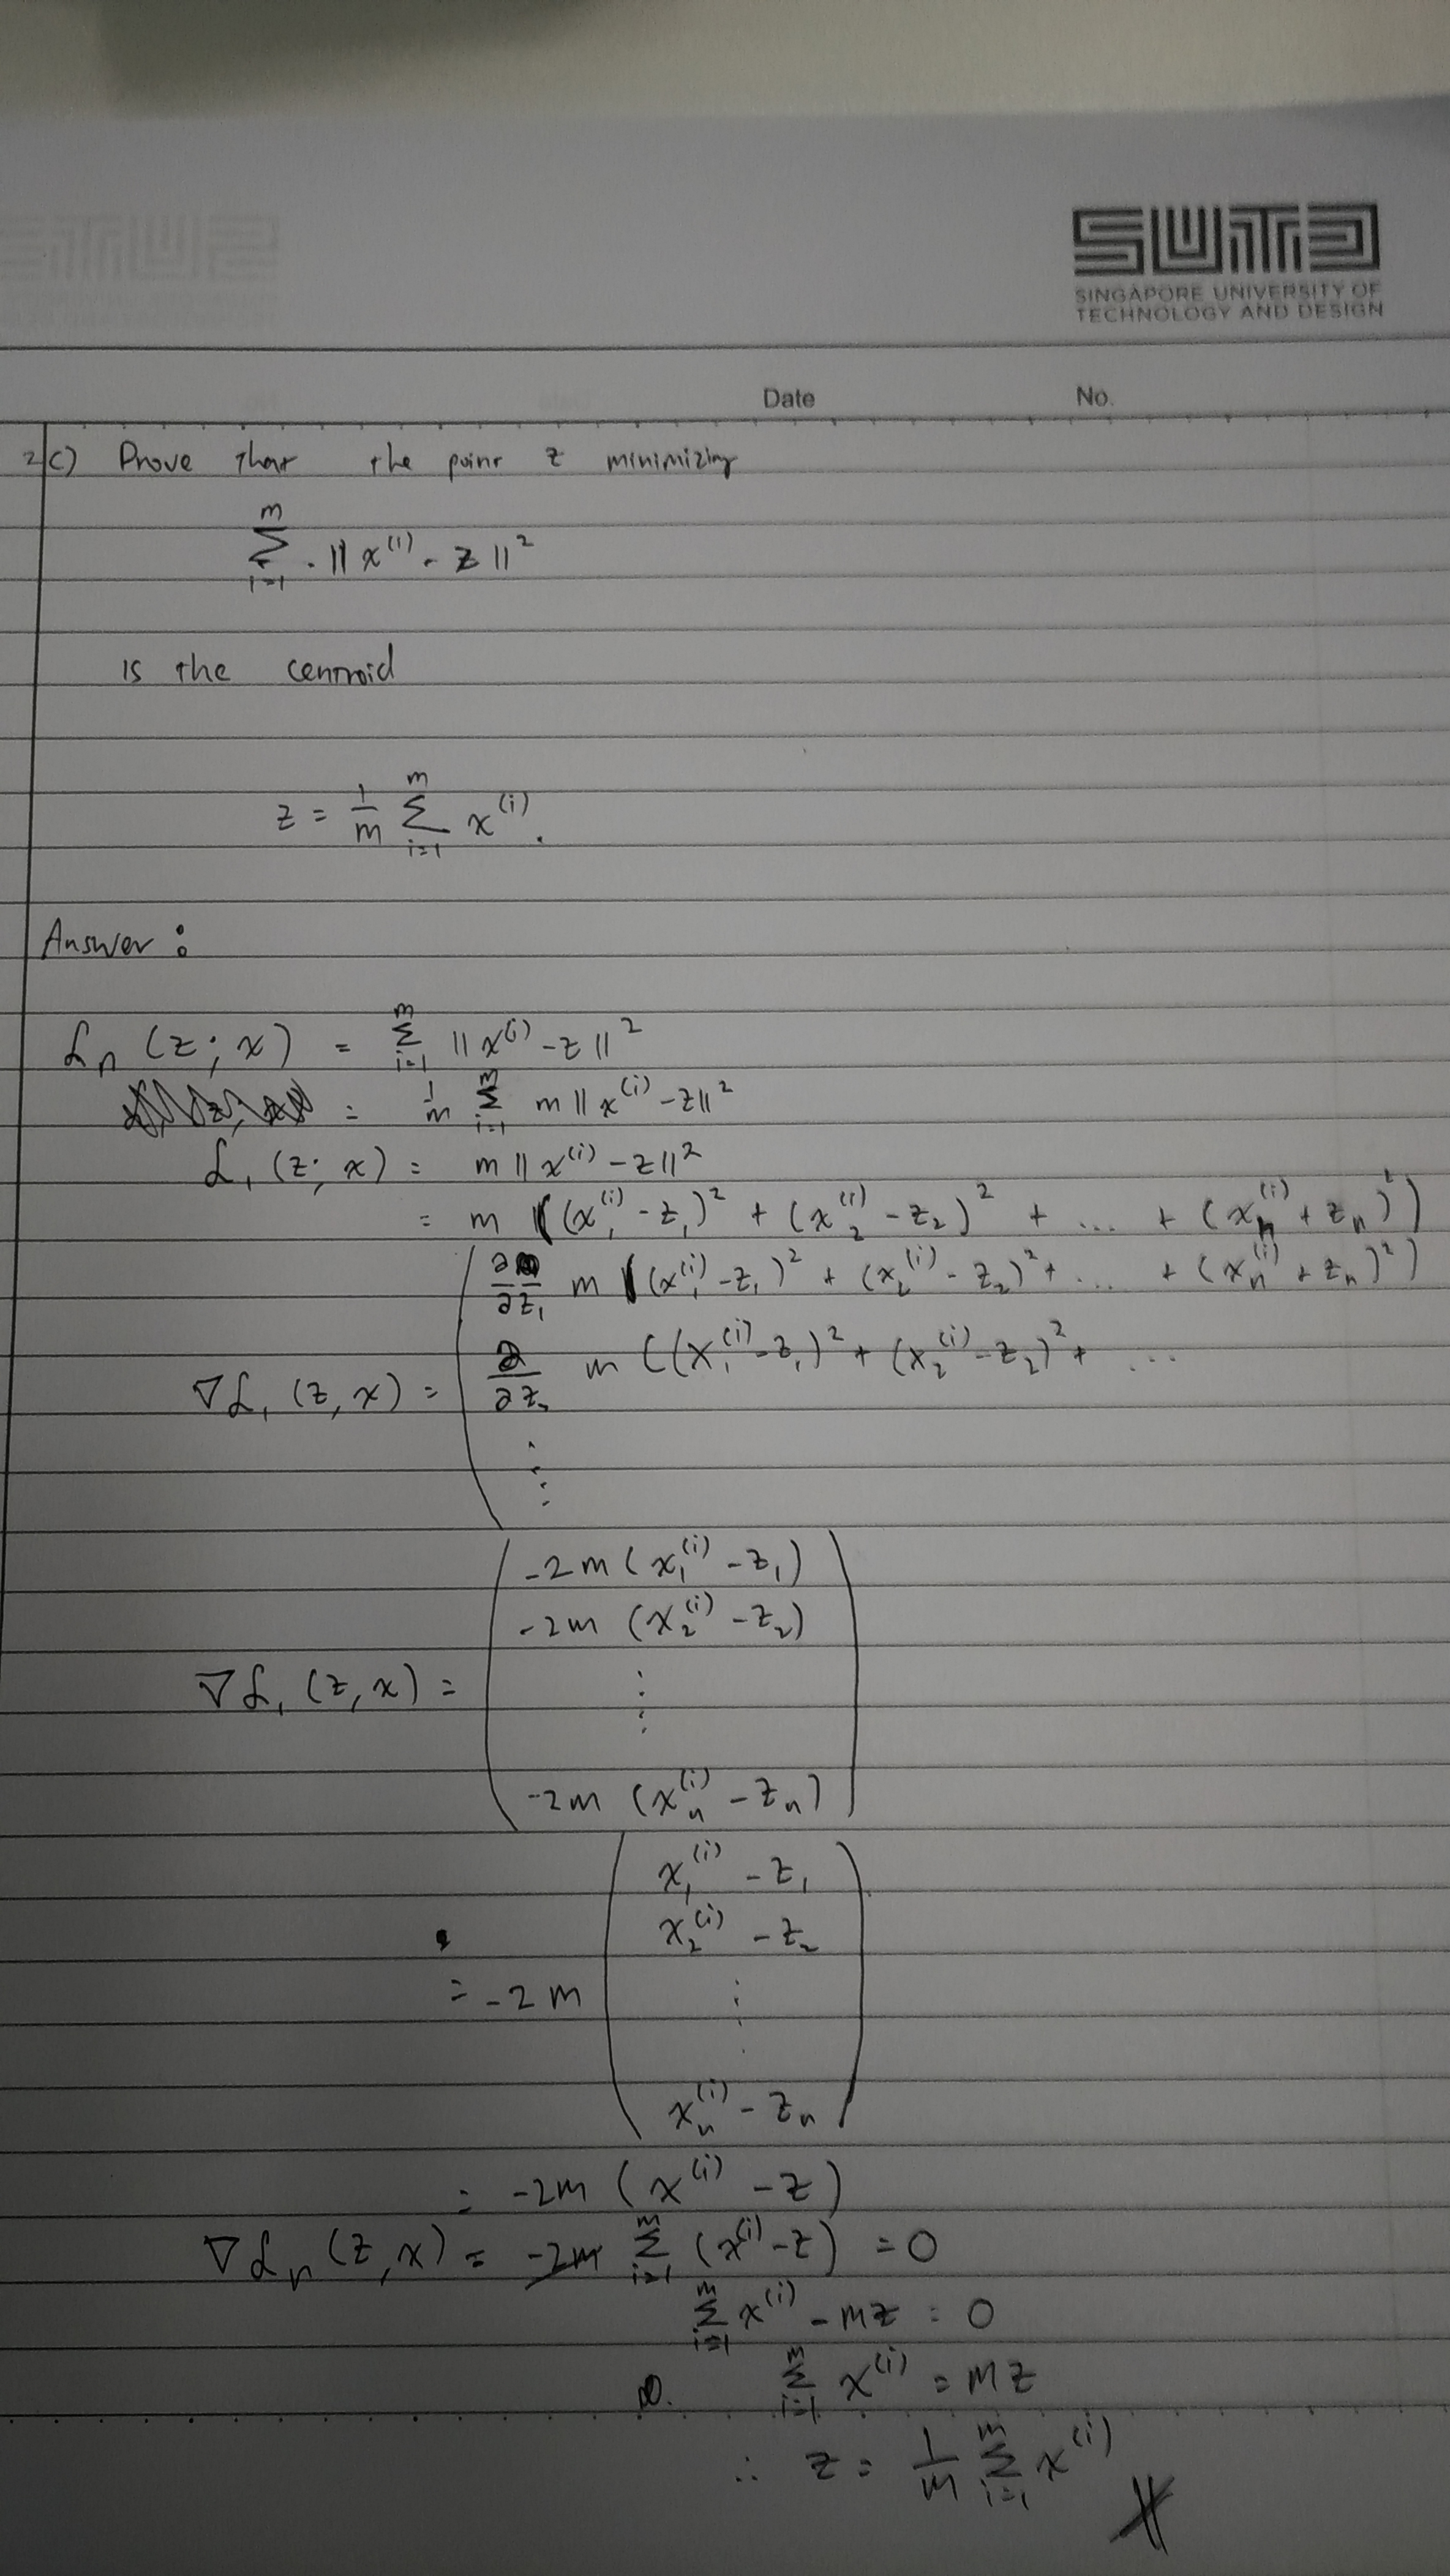
\includegraphics{prove.jpg}
\caption{Answer}
\end{figure}


    % Add a bibliography block to the postdoc
    
    
    
    \end{document}
